\documentclass[a4paper, 12pt, diplomski]{etfcyr}

\usepackage[serbianc]{babel}
\usepackage{fontspec}
\usepackage{polyglossia}
\usepackage[document]{ragged2e}
\usepackage{indentfirst}
\usepackage{enumitem}
\usepackage{scrextend}
\usepackage{etoolbox}
\usepackage{graphicx}
\usepackage{textcomp}
\usepackage{multicol}
\usepackage{float}
\usepackage{wrapfig}
\usepackage{listings}
\usepackage{array}
\usepackage{caption}


\DeclareGraphicsExtensions{.pdf,.png,.jpg}

\addtokomafont{labelinglabel}{\textbf}

\setdefaultlanguage[script=Cyrillic]{serbian}
%\newfontfamily{\cyrillicfont}{Times New Roman}

\setmainfont{Times New Roman}
\setsansfont{Arial}
\setmonofont{PragmataPro}

\renewcommand*\contentsname{Садржај}

\newcommand{\indentfirstparagraphon}{
	\renewenvironment{justify}{%
		\trivlist
		\justifying
		\itemindent\JustifyingParindent
	\item\relax
	}{
		\endtrivlist
	}
}

\newcommand{\indentfirstparagraphoff}{
	\renewenvironment{justify}{%
		\trivlist
		\justifying
		\item\relax
	}{
		\endtrivlist
	}
}

\makeatletter
\gdef\tshortstack{\@ifnextchar[\@tshortstack{\@tshortstack[c]}}
\let\@tshortstack\@shortstack
\patchcmd\@tshortstack\vbox\vtop{}{}
\makeatother

\makeatletter
\def\@makechapterhead#1{%
	\vspace*{50\p@}%
	{\parindent \z@ \raggedright \normalfont
		\interlinepenalty\@M
		\Huge\bfseries  \thechapter.\quad #1\par\nobreak
		\vskip 20\p@
	}}
\makeatother

\indentfirstparagraphon

\addto\captionsserbian{%
	\renewcommand{\bibname}%
	{Литература}%
}

\addto\captionsserbian{%
	\renewcommand{\lstlistlistingname}%
	{Списак листинга}%
}

\addto\captionsserbian{%
	\renewcommand{\lstlistingname}%
	{Листинг}%
}


\def\code#1{\texttt{#1}}
\def\quote#1{„#1“}

\lstset{basicstyle=\footnotesize\ttfamily,tabsize=4,captionpos=t,frame=tb}
\captionsetup[lstlisting]{font={rm}}

\setlength{\parindent}{4em}
\setlength{\JustifyingParindent}{4em}

\title{Паметна соба - контрола уласка}
\author{Топлица Танасковић}
\indeks{164/1996}
\date{септембар 2016.}
\mentor{Проф. др Драган Бојић}
\predmet{Системско програмирање}

\begin{document}
%	\sloppy
	\maketitle

	\thispagestyle{empty}
	\vspace*{\fill}
	\begin{center}
			\textit{\thanks{Овај рад посвећујем својим родитељима и супрузи која је имала разумевања и стрпљења за моју одсутност током рада на њему.}}
	\end{center}
	\vspace*{\fill}

	\begin{abstract}
		\begin{justify}
			У овом раду је изложен проблем прављења распореда коришћења лабораторија са контролом уласка. Објашњени су најчешћи сценарији који задају доста проблема и предложено је софтверско решење као испомоћ.
		\end{justify}
	\end{abstract}

	\begin{keywords}
		Дипломски радови, контрола приступа, програмирање, C++
	\end{keywords}
	\tableofcontents
	\listoffigures
	\listoftables
	\lstlistoflistings

	\chapter{Увод}

		\begin{justify}
			Прављење распореда рада у факултетским лабораторијама је велики проблем са којим особље мора стално да се носи. Број студената и активности које морају да се обаве је огроман, а факултет има ограничен број лабораторија и радних места у њима. Ово представља проблем за људе који су одговорни распоред јер морају да воде рачуна о много активности, студената и термина, док у исто време покушавају да избегну преклапања или конфликте.

			Проблем можемо сагледати са два аспекта, први је прављење распореда, а други је безбедност. Како је већ напоменуто, факултет има ограничен број лабораторија одређеног капацитета док је број студената са својим задацима и обавезним активностима огроман.

			Прављење распореда рада са дозволом уласка је врло тешко јер захтева праћење великог броја, како студената, тако и активности како би се обезбедило да нема преклапања. Радити ово ручно није оптимално и подложно је грешкама што може да доведе до разних преклапања, промена распореда у задњи час и многих других проблема. Без обзира што многе активности нису обавезне доста њих је у исто време обавезно и врло битно за студенте, као што су рецимо колоквијуми или испити. Овакве активности не би смеле да се одлажу нити прекидају улажењем других особа у просторију.

			Што се тиче безбедности, неке лабораторије осим што имају деликатну и скупу, имају и врло опасну опрему која може услед погрешног руковања да начини огромну штету или чак нанесе опасне повреде. Због овога би требало ограничити приступ тј. улаз у неке од лабораторија како би се избегле у крајњим случајевима и несагледиве последице.
		\end{justify}

	\chapter{Дискусија}
		\begin{justify}
			У овом поглављу ће зарад лакшег сагледавања проблема поред дефиниција разних појмова који се помињу даље у тексту, бити дефинисани и начини, односно сценарији, коришћења лабораторија.
		\end{justify}
		
		\section{Начини коришћења лабораторија}

			\begin{justify}
				Број начина на које једна лабораторија може да се користи углавном зависи од њене намене. Међутим, без обзира на намену лабораторије могу се уочити четири најчешћа начина на које се оне користе. Да би се целокупан проблем прецизније дефинисао, у овом одељку ће се дискутовати понаособ сваки од начина коришћења.
			\end{justify}

			\subsection{Дефиниције}

				\begin{justify}
					Пре него што будемо могли да опишемо начине на које се лабораторије користе, морамо увести неке дефиниције и успоставити релације међу њима.
				\end{justify}

				\begin{labeling}{\smash{\tshortstack[l]{Корисник\\лабораторије}}}
					\indentfirstparagraphoff

					\item [Активност] 
						\begin{justify}
							Активност је било који процес који се одвија у лабораторији, без обзира на његово трајање, евентуалну периодичност или конкретан тип.
						\end{justify}

					\item[\smash{\tshortstack[l]{Тип\\активности}}]
						\begin{justify}
							Тип активности ближе дефинише активност, и одређује њен приоритет у односу на друге. Постоје следећи типови активности.
							\begin{enumerate}[noitemsep]
								\item Испит
								\item Колоквијум
								\item Предавања или вежбе
								\item Лабораторијске вежбе
								\item Посебни догађаји
								\item Индивидуални рад
							\end{enumerate}
						\end{justify}

					\item[\smash{\tshortstack[l]{Приоритет\\активности}}]
						\begin{justify}
							Приоритет активности одређује да ли је дозвољен улаз у просторију уколико се у њој преклапају активности, а једна од њих је битнија. Не желимо да допустимо да људи улазе и излазе из просторије док је у току испит. Приоритет активности је дефинисан типом активности како је наведено у претходној дефиницији.\\
							Индивидуални рад је посебан случај. Приликом заказивања такве активности може се посебно дозволити улазак без обзира на то да ли се у просторији већ одвија нека активност вишег приоритета. Ово се углавном користи за студенте који раде дипломски или неки други важан пројекат.
						\end{justify}

					\item[\smash{\tshortstack[l]{Корисник\\лабораторије}}]
						\begin{justify}
							Корисник лабораторије је било која особа којој се може дозволити улаз у лабораторију. Постоје две врсте корисника:
							\begin{enumerate}[noitemsep]
								\item Професор
								\item Студент
							\end{enumerate}
							Можда би се могао увести и \quote{студент демонстратор} као засебан тип корисника, али како он нема посебна права, довољно је да буде члан листе која је маркирана као листа демонстратора како би могао да приступи лабораторији у заказаном термину без обзира да ли је нека друга активност у току.
						\end{justify}

					\item [Листа]
						\begin{justify}
							Листе су групе особа, односно корисника, лабораторија које служе зарад лакше манипулације током заказивања активности и доделе права уласка у лабораторију. Постоје три врсте листи:
							\begin{enumerate}[noitemsep]
								\item Системске листе
								\item Трајне листе
								\item Привремене листе
							\end{enumerate}
							Привремене листе имају свој рок трајања и након тога се аутоматски бришу из система. Системске листе су посебан случај трајних листа, оне се не могу мењати и о њима систем сам води рачуна. Пример системске листе је листа студената друге године.
						\end{justify}

					\item [Просторија]
						\begin{justify}
							Просторија је било која лабораторија, кабинет или учионица у којој се одвијају неке активности и за коју желимо да имамо контролу уласка.
						\end{justify}

					\item[\smash{\tshortstack[l]{Системски\\корисник}}]
						\begin{justify}
							Системски корисници су особе које могу да врше подешавање система, имају контролу над свим подацима у систему и приступ извештајима. Ови корисници су подељени у три улоге:
							\begin{enumerate}[noitemsep]
								\item Супер корисник
								\item Администратор
								\item Менаџер
							\end{enumerate}
							Шта је којој улози дозвољено да ради биће дефинисано касније када се буду дефинисале компоненте система.
						\end{justify}
					\indentfirstparagraphon
				\end{labeling}

			\subsection[Сценарио 1]{Испити и колоквијуми}
				\begin{justify}
				Ово је вероватно најбитнији сценарио. Активности дефинисане овим сценариом се обично не понављају и имају тачно дефинисан датум и време почетка као и трајање. Оваквим активностима се обично додељује једна листа студената, али није искључено да се додели и више. Такође овакве активности се најчешће одвијају у више просторија паралелно.
				\end{justify}

			\subsection[Сценарио 2]{Предавања или вежбе}
				\begin{justify}
					Предавања и вежбе су пример активности које се понављају на недељном нивоу један дужи временски период, и одвијају се у једној просторији. Ову врсту активности обично посећује иста група људи, прецизније студенти који слушају дати предмет, или ако је предмет обавезан онда сви студенти дате године студија.
				\end{justify}

			\subsection[Сценарио 3]{Лабораторијске вежбе}
				\begin{justify}
					Лабораторијске вежбе су пример активности код којих поред студената и професора можемо имати и студенте демонстраторе. Студентима демонстраторима би требало такође дозволити несметан улаз и то се лако може постићи додавањем нове листе која ће садржати демонстраторе у систем, и додељивањем те листе активности. Овакве активности се најчешће изводе у једној просторији, али није немогуће да се одвијају паралелно у више.
				\end{justify}

			\subsection[Сценарио 4]{Посебни догађаји}
				\begin{justify}
					У овакве активност превасходно спадају јавна предавања, презентације и конференције. У оваквим случајевима у просторијама се увек налази неко од особља као што су предавачи, те контрола приступа није потребна. Овакве активности не захтевају да имају додељену листу.
				\end{justify}

			\subsection[Сценарио 5]{Индивидуални рад}
				\begin{justify}
					Посебна карактеристика ове врсте активности је то што она може, ако је дефинисано, да дозволи улаз у просторију без обзира да ли је нека друга активност у току. Оваква активност захтева листу студената, којој може да припада и само један студент. Овакве активности се најчешће одобравају студентима који раде дипломски или неки други важан рад, а имају потребу за опремом која се налази у лабораторијама.
				\end{justify}

		\section{Посебне напомене}
			\begin{justify}
				Уколико је неопходно, могуће је одређеним студентима забранити улазак у неку просторију. Студенти којима је улаз забрањен неће моћи да уђу у дату просторију иако су на листи за активност која се одвија у њој.
			\end{justify}

	\chapter{Предлог решења}
		\begin{justify}
			Ово поглавље излаже предлог решења, даје ближи опис и улогу сваке од компоненти система и дефинише протоколе комуникације између сваке од њих. Такође, дат је и опис комуникације са другим системима у виду увоза и извоза података.
		\end{justify}

		\section{Уопштени преглед система}
			\begin{justify}
				Услед саме природе проблема, као и потребе да компоненте комуницирају на поуздан и безбедан начин, систем мора да буде модуларан са прецизно дефинисаним протоколима комуникације и обраде грешака. Уопштен дијаграм система дат је на слици испод.

				\begin{figure}[h]
					\begin{center}
						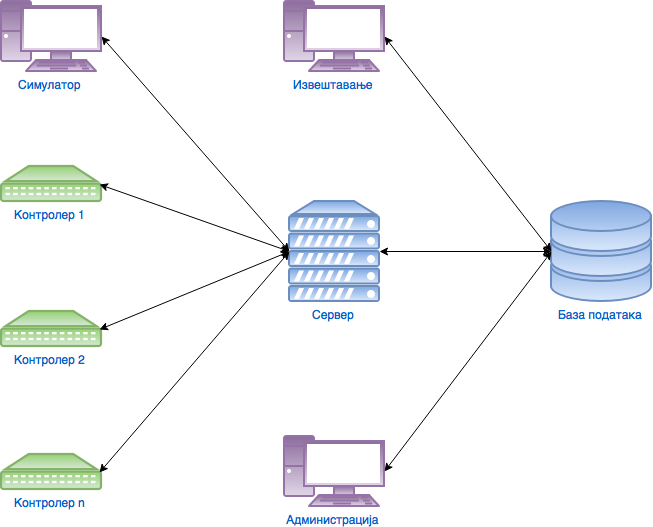
\includegraphics[scale=0.47]{SystemOverview.png}
					\end{center}
					\caption{Дијаграм система}
					\label{figure:1}
				\end{figure}

				Са дијаграма на слици \ref{figure:1} лако можемо уочити да постоје три различите врсте компоненти. Плаве су чисто софтверске компоненте које раде на серверу, љубичасте су такође софтверске компоненте, али раде на локалним рачунарима, док зелене компоненте представљају микроконтролере са припадајућом хардверско-софтверском подршком.
			\end{justify}

		\section{Компоненте система}

			\subsection{База података}
				\begin{justify}
					Сервер базе података је одговоран за свеобухватно похрањивање података. Посебних хардверских захтева нема, сем да постоји довољно меморије и складишног простора на диску. Сервер базе података који се користи у овом решењу је PostgreSQL издање 9.2, а може се користити и новија верзија.
					\begin{figure}[h]
						\begin{center}
							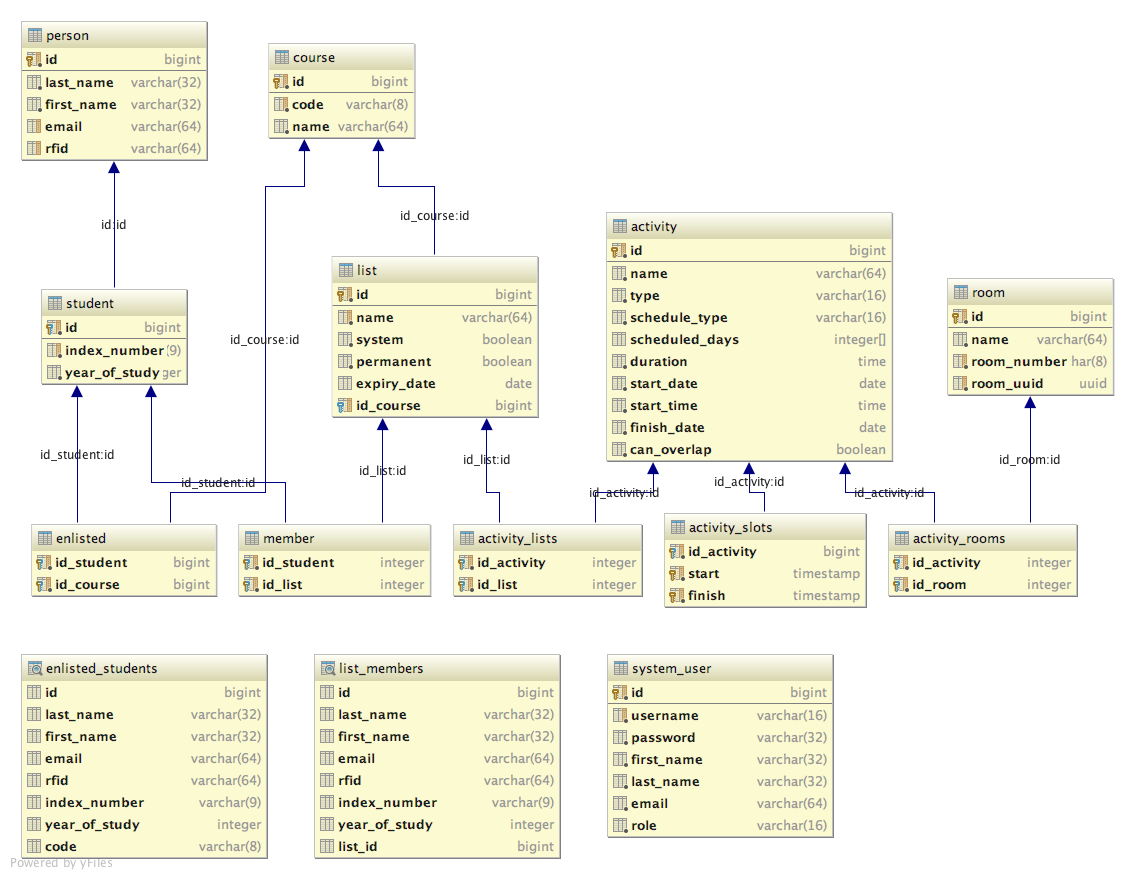
\includegraphics[scale=0.25]{DatabaseDiagram.png}
						\end{center}
						\caption{Дијаграм базе података}
						\label{figure:2}
					\end{figure}
				\end{justify}
				
			\subsection{ПаСо сервер}
				\begin{justify}
					\quote{ПаСо} сервер је централна компонента система. Његова одговорност је да комуницира са контролерима просторија и са симулатором као алатом за тестирање. Сам сервер је имплементиран као стандардни UNIX сервер који прихвата TCP конекције на порту који је одређен подешавањима. Овај сервер није пасивна компонента која само чека захтеве и обрађује их, већ периодично шаље и \quote{јеси ли жив} сигнале пријављеним контролерима и симулаторима. Такође, одговоран је и за слање података које би контролери требало да користе уколико дође до прекида у комуникацији, као и за брисање листи којима је истекао рок. Формат комуникације, порука и података за случај прекида саме комуникације биће дефинисан касније.
					Илустрација рада сервера дата је на слици \ref{figure:3}.
					\begin{figure}[h]
						\begin{center}
							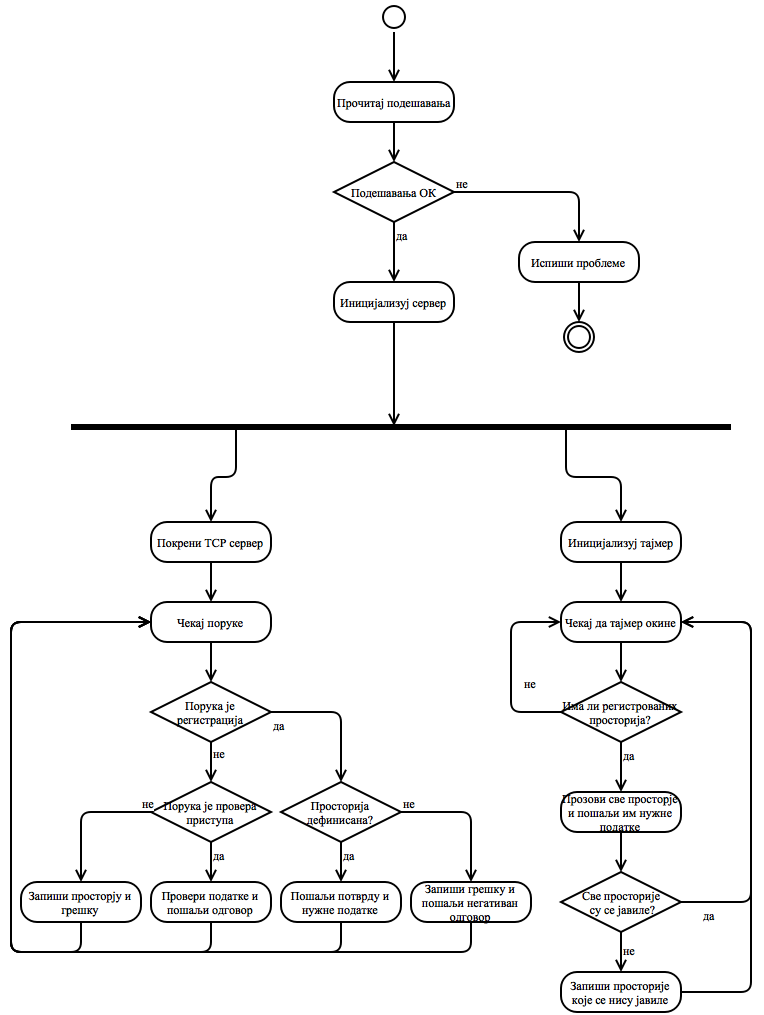
\includegraphics[scale=0.35]{ServerWorkflow.png}
						\end{center}
						\caption{Дијаграм рада сервера}
						\label{figure:3}
					\end{figure}
				\end{justify}

			\subsection{Администрација}
				\begin{justify}
					Ова компонента је одговорна за комплетну администрацију целог система, почев од управљања корисницима и просторијама па све до заказивања активности. У административном програму постоје следећи модули:

					\begin{labeling}{\smash{\tshortstack[l]{Управљање\\активностима}}}
						\indentfirstparagraphoff

						\item[\smash{\tshortstack[l]{Управљање\\системским\\корисницима}}]
							\begin{justify}
								Овај модул служи за одржавање листе корисника система. Корисници дефинисани у овом модулу немају никаве везе са корисницима лабораторија и служе искључиво за администрацију система. Сви корисници су распоређени у више улога, о чему ће бити речи касније.
							\end{justify}

						\item[\smash{\tshortstack[l]{Управљање\\просторијама}}]
							\begin{justify}
								Поред уношења нових просторија и додељивања јединственог идентификатора, управљање просторијама подразумева и одржавање листе студената којима је забрањен улаз за сваку просторију понаособ.
							\end{justify}

						\item[\smash{\tshortstack[l]{Управљање\\предметима}}]
							\begin{justify}
								Овај део се бави одржавањем података о предметима на факултету и подржава увоз података из CSV датотека. Постоје две врсте података које се могу увозити. Прва је сама листа предмета са припадајућим подацима, а друга представља податке о студентима који слушају одређени предмет. Формати CSV датотека за обе врсте података биће дати касније у засебном одељку.
							\end{justify}

						\item[\smash{\tshortstack[l]{Управљање\\студентима}}]
							\begin{justify}
								Овај модул служи за одржавање комплетне листе студената. Поред стандардних података о студенту као што је број индекса, име и презиме, електронска пошта итд. у овом модулу се уноси и РФИД студентских картица које омогућавају студентима приступ факултетским просторијама. Уколико је потребно студенту забранити приступ свим просторијама где се врши контрола уласка, довољно је само обрисати РФИД из његових личних података и он више неће моћи своју картицу да користи за откључавање врата.
								За сваког студента се могу видети детаљи као што су подаци о томе које предмете слуша и којих је листи члан.
								Као и претходни модул, и овај подржава увоз података о студентима из CSV датотека.
							\end{justify}

						\newpage

						\item[\smash{\tshortstack[l]{Управљање\\наставним\\особљем}}]
							\begin{justify}
								Управљање наставним особљем је у суштини исто као и управљање студентима, са разликом што наставно особље не припада ни једној листи, већ се њима увек дозвољава улазак у просторије без обзира да ли се нека активност одвија или не. Као и код студената, и овде је довољно обрисати РФИД из података да би се онемогућио улазак у просторије се контролом приступа. Ово је згодно уколико дође до губљења или крађе картице.
							\end{justify}

						\item[\smash{\tshortstack[l]{Управљање\\листама}}]
							\begin{justify}
								Сврха овог дела је да пружи решење за лакше управљање правима приступа, као и за бољу прегледност груписањем студената у листе. Такође, обезбеђен је и увоз података у виду чланова за сваку листу. Када су у питању системске листе, њихова измена или брисање није могуће пошто о њима бригу води сам систем.
							\end{justify}

						\item[\smash{\tshortstack[l]{Управљање\\активностима}}]
							\begin{justify}
								Ово је најсложенији и вероватно најбитнији део администрације, пошто се поред креирања активности бави и њиховим заказивањем које може бити различито у зависности од потребе. Свака активност садржи мноштво података те се зарад боље прегледности уређивање одвија у корацима путем чаробњака. Што се тиче заказивања активности подржана су два начина, заказивање једног тачно одређеног термина, и заказивање на одређени временски период са понављањем на недељном или месечном нивоу. У оба случаја где се активност понавља потребно је одабрати тачне дане понављања у недељи или месецу. Без обзира на начин заказивања, приликом снимања активности врши се провера преклапања термина са већ заказаним активностима. Код ове провере, постојеће активности типа \quote{Индивидуални рад} се не узимају у обзир.
							\end{justify}

						\end{labeling}
				\end{justify}

			\newpage

			\subsection{Приступ модулима у зависности од системске улоге}
				\begin{justify}
					Матрица приступа административном модулу у зависности од улоге додељене системском кориснику дата је у табели \ref{table:1}.
				\end{justify}
				\begin{table}[H]
					\centering
					\begin{tabular}{ c||c|c|c }
						Модул\textbackslash Улога & Супер корисник & Администратор & Менаџер \\
						\hline\hline
						Системски корисници & да & да & не \\
						Просторије & да & да & не \\
						Предмети & да & не & да \\
						Студенти & да & не & да \\
						Наставници & да & не & да \\
						Листе & да & не & да \\
						Активности & да & не & да \\
						\hline
					\end{tabular}
					\caption{Приступ модулима у зависности од системске улоге}
					\label{table:1}
				\end{table}

			\subsection{Извештавање}
				\begin{justify}
					Компонента задужена за извештавање није засебна, већ је интегрисана у административни модул. Понуђена су три извештаја, два се односе на безбедност, то је извештај улазака у одабрану просторију и сви уласци одређене особе у било коју од просторија, док трећи даје преглед заузећа собе. Извештаји везани за просторије се налазе у одељку за управљање просторијама, док се извештај за о уласцима особа у просторија налазе у одељцима за управљање студентима односно наставним особљем.
				\end{justify}

			\subsection{Контролери просторија}
				\begin{justify}
					Ова компонента са припадајућим хардвером и софтвером служи да контролише аутоматску браву на вратима просторија, чита РФИД картице или токене и комуницира са сервером. Сваки контролер, пре него што може да се стави у употребу мора да се подеси и да се одговарајућа просторија унесе у систем путем административног модула. Подешавање подразумева да се у контролер унесе јединствени идентификатор просторије који је изгенерисан у административном модулу, као и адреса \quote{ПаСо} сервера.
				\end{justify}



				\subsubsection*{Опис рада контролера просторије}

					\begin{figure}[h]
						\begin{center}
							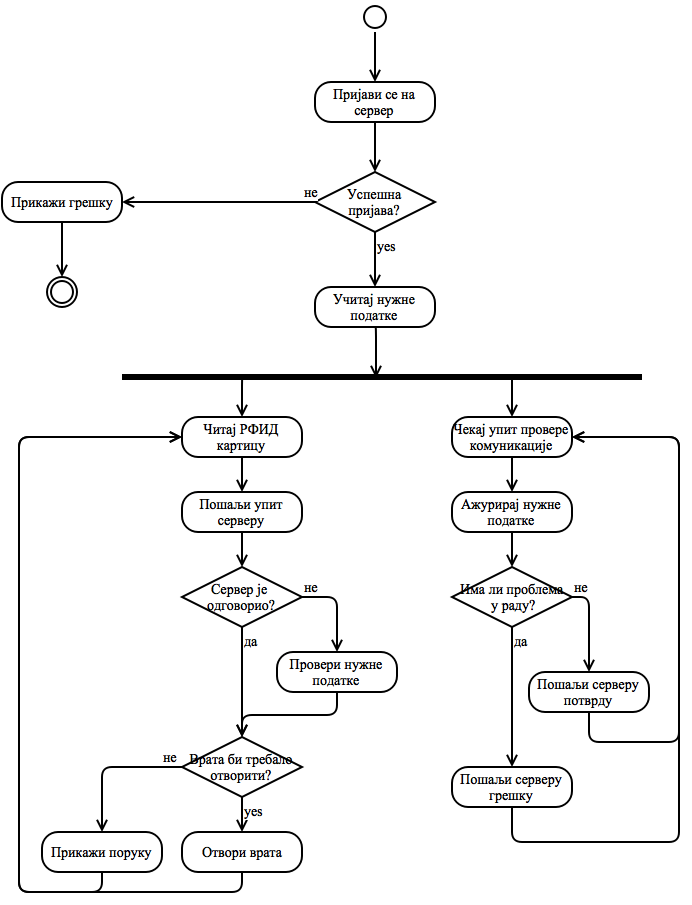
\includegraphics[scale=0.35]{RoomControllerWorkflow.png}
						\end{center}
						\caption{Дијаграм рада контролера}
						\label{figure:4}
					\end{figure}
					\begin{justify}
						Као што се може видети на слици \ref{figure:4}, по укључивању напајања, контролер би требало да се региструје на сервер. Ово је неопходно из разлога што сервер мора да зна адресу контролера како би могао периодично да шаље захтеве којима ће да проверава да ли комуникација са контролером није случајно прекинута. Поред захтева којима се проверава стање комуникације, сервер мора контролеру периодично да шаље податке који су му неопходни за рад уколико до прекида комуникације ипак дође. Ови подаци не представљају ништа друго до РФ идентификаторе картица и токена наставног особља, како би у случају да нема комуникације они могли несметано да улазе у просторије или отворили врата особљу задуженом за одржавање опреме.
						По регистрацији, контролер чека на читање РФИД картице или токена, након чега шаље серверу упит да ли би требало да отвори врата датој особи. Паралелно са тим контролер слуша на TCP порту како би могао да одговори на серверове провере стања комуникације и прихвати податке за рад у случају прекида исте. Уколико услед било ког разлога контролер није пријављен на сервер, рецимо био је пријављен па је сервер поново покренут, сервер ће у одговору на упит права приступа послати и нотификацију контролеру да мора да уради нову регистрацију, а приступ ће бити дат само наставном особљу.
						Детаљан формат комуникације између сервера и контролера биће дат у засебном одељку.
					\end{justify}

			\subsection{Симулатор}
				\begin{justify}
					Симулатор је компонента чија сврха је да убрза развој и потпомогне тестирање како сервера тако и контролера просторија. Такође, може се користити и за проверу понашања система под различитим околностима. Симулатор је написан као класична интерактивна десктоп апликација и има исти алгоритам рада као и контролер просторије. Главна улога симулатора, поред тестирања сервера, јесте да особама које раде на развоју хардверских контролера просторија да увид у формат и протокол комуникације, како обрађивати грешке, итд. Све поруке које се размењују између симулатора и сервера могу се видети директно у самом симулатору користећи JSON нотацију. Поред симулације читања РФИД картица и токена, компонента може да симулира и прекид комуникације са сервером.
				\end{justify}

		\newpage

		\section{Протокол комуникације и формати порука}
			\begin{justify}
				Због лакшег развоја и отклањања проблема, како у току развоја тако и за време експлоатације система, све поруке које се размењују између компоненти су у JSON формату.
			\end{justify}

			\subsection{Безбедност комуникације}
				\begin{justify}
					Да би се повећала безбедност система и спречило било какво ослушкивање саобраћаја сва комуникација је осигурана SSL TLS v1 протоколом.
				\end{justify}
			
			\subsection{Основни формат поруке}
				\begin{justify}
					Свака порука која се шаље, на почетку увек има два бајта која означавају њену дужину, а након њих следи сама порука у JSON формату. Дужина прослеђена у прва два бајта не укључује та два бајта, и уколико се послата дужина поруке и њена стварна, тј. прочитана, дужина не слажу, порука ће се сматрати неисправном и биће игнорисана. Све поруке које долазе од контролера или симулатора морају да имају \quote{roomid} и \quote{operation} поља уз додатак других ако је то неопходно. Сваки одговор на поруку мора имати исту вредност у пољу \quote{operation}.
					За опис свих порука користи се \quote{JSON Schema} формат о коме се може прочитати на \textbf{http://json-schema.org} интернет страници.
				\end{justify}

			\newpage

			\subsection{Регистрација контролера или симулатора на сервер}
				\begin{justify}
					Поруке које контролери или симулатори шаљу да би се регистровали на систем морају да одговарају следећој JSON шеми:
					\begin{lstlisting}[caption=Формат захтева за регистрацију]
{
	"$schema": "http://json­schema.org/draft­04/schema#",
	"description": "The room registration request",
	"type": "object",
	"properties": {
		"room­id": { "type": "string" },
		"operation": { "type": "string" }
	},
	"required" : ["room­id", "operation"]
}
					\end{lstlisting}
					Вредност поља \quote{operation} за поруке регистрације на сервер је увек \quote{register}.
					Очекиван одговор од сервера је у следећем формату:
					\begin{lstlisting}[caption=Формат одговора на захтев за регистрацију]
{
	"$schema": "http://json­schema.org/draft­04/schema#",
	"description": "The room registration response",
	"type": "object",
	"properties": {
	"room­id": { "type": "string" },
	"operation": { "type": "string" },
	"success": { "type": "boolean" },
	"port": { "type": "integer" },
	"emergency­data" : {
		"type": "array",
		"items": { "type": "string" }
		}
	}
	"required": [ "room­id", "operation", "success" ]
}
					\end{lstlisting}
				\end{justify}

			\newpage

			\subsection{Провера комуникације и статуса контролера}
				\begin{justify}
					Ове поруке шаље сервер како би проверио да комуникација није прекинута, као и да добије повратну информацију од контролера о његовом стању. Формат ове поруке је следећи:
					\begin{lstlisting}[caption=Формат захтева провере комуникације и статуса]
{ 
	"$schema": "http://json­schema.org/draft­04/schema#",
	"description": "Are you alive request",
	"type": "object",
	"properties": {
		"room­id": { "type": "string" },
		"operation": { "type": "string" },
		"emergency­data" : {
			"type": "array",
			"items": { "type": "string" }
		}
	}
	"required": [ "room­id", "operation" ]
}
					\end{lstlisting}
					Вредност поља \quote{operation} је увек \quote{ping}.
					Очекивани одговор од контролера или симулатора је следећи:
					\begin{lstlisting}[caption=Формат одговора на захтев провере комуникације и статуса]
{
	"$schema": "http://json­schema.org/draft­04/schema#",
	"description": "Are you alive response",
	"type": "object",
	"properties": {
		"room­id": { "type": "string" },
			"operation": { "type": "string" },
			"response": { "type": "boolean" },
			"fault": { "type": "string" }
		}
	"required": [ "room­id", "operation", "response" ]
}
					\end{lstlisting}
					Вредност поља \quote{response} може да буде \quote{false}, у том случају мора постојати и поље \quote{fault} које садржи разлог отказа контролера, на пример, неисправан хардвер, и сервер ће уписати ту поруку у свој дневник. У случају да је све уреду поље \quote{response} има вредност \quote{true} и поље \quote{fault} није обавезно.
				\end{justify}

			\newpage

			\subsection{Провера права приступа}
				\begin{justify}
					Ову поруку шаље контролер по очитавању картице да би са сервером проверио да ли би особу требало пустити у просторију. Формат је следећи:
					\begin{lstlisting}[caption=Формат захтева за проверу права приступа]
{
	"$schema": "http://json­schema.org/draft­04/schema#",
	"description": "The access permission query",
	"type": "object",
		"properties": {
			"room­id": { "type": "string" },
			"operation": { "type": "string" },
			"rfid" : { "type": "string" }
		}
	"required": [ "room­id", "operation", "rfid" ]
}
					\end{lstlisting}
					Поље \quote{operation} је \quote{access}. Одговор је у следећем формату:
					\begin{lstlisting}[caption=Формат одговора на захтев за проверу права приступа]
{
	"$schema": "http://json­schema.org/draft­04/schema#",
	"description": "The access permission query response",
	"type": "object",
		"properties": {
			"room­id": { "type": "string" },
			"operation": { "type": "string" },
			"granted" : { "type": "boolean" },
			"reregister" : { "type": "boolean" }
		}
	"required": [ "room­id", "operation", "granted" ]
}
					\end{lstlisting}
					Уколико вредност поља \quote{granted} није \quote{true} контролер неће отворити-откључати врата.
				\end{justify}

		\newpage

		\section{Увоз и извоз података}
			\begin{justify}
				За увоз и извоз података користи се искључиво CSV формат. Структура CSV датотеке мора у потпуности да одговара форматима који су дефинисани у овом одељку, не смеју садржати празне редове нити било какве друге податке. Подаци који се могу увозити су:
				\begin{enumerate}[noitemsep]
					\item Подаци о предметима.
					\item Подаци о студентима.
					\item Листе студената који слушају одређени предмет.
					\item Произвољне листе студената, као на пример списак за полагање испита.
				\end{enumerate}
				Подаци који се могу извозити су извештаји и то:
				\begin{enumerate}[noitemsep]
					\item Списак особа које су улазиле у одређену просторију у датом периоду.
					\item Списак просторија у које је одређена особа улазила у датом периоду.
					\item Извештај о заузећу одабране просторије.
				\end{enumerate}
			\end{justify}

			\subsection{Формат података за увоз}
				\begin{justify}
					Формат CSV датотека које представљају списак студената који слушају неки предмет, или рецимо списак за лабораторијске вежбе или испит је у потпуности произвољан уз ограничење да број индекса мора стајати на почетку, остатак реда се игнорише.
					Формати датотека за увоз осталих подржаних података су дати у табелама испод.
				\end{justify}
				\begin{table}[H]
					\centering
					\begin{tabular}{ c l l }
						Колона & Значење & Тип \\
						\hline
						1. & шифра предмета & текст \\
						2. & име предмета & текст \\
					\end{tabular}
					\caption{Формат за увоз података о предметима}
					\label{table:2}
				\end{table}
				\begin{table}[H]
					\centering
					\begin{tabular}{ c l l }
						Колона & Значење & Тип \\
						\hline
						1. & име & текст \\
						2. & презиме & текст \\
						3. & ел. пошта & текст \\
						4. & број индекса у формату гггг/бббб & текст \\
						5. & година студија & цео број \\
					\end{tabular}
					\caption{Формат за увоз података о студентима}
					\label{table:3}
				\end{table}

			\newpage

			\subsection{Формат за извоз података}
				\begin{justify}
					Извештаји о уласцима особа у одређену просторију или уласцима одређене особе за неки период су идентични у свом формату и дати су у табели \ref{table:4}, док је формат извештаја о заузећу неке просторије дат у табели \ref{table:5}.
					\begin{table}[H]
						\centering
						\begin{tabular}{ c l l }
							Кол. & Значење & Тип \\
							\hline
							1. & број просторије & текст \\
							2. & број индекса или интерни број запосленог & текст \\
							3. & име & текст \\
							4. & презиме & текст \\
							5. & датум и време & ИСО 8061 формат \\
						\end{tabular}
						\caption{Формат извештаја о уласцима}
						\label{table:4}
					\end{table}
					\begin{table}[H]
						\centering
						\begin{tabular}{ c l l }
							Кол. & Значење & Тип \\
							\hline
							1. & број просторије & текст \\
							2. & активност која је у питању & текст \\
							3. & почетак активности & ИСО 8061 формат \\
							4. & крај активности & ИСО 8061 формат \\
						\end{tabular}
						\caption{Формат извештаја о заузећу просторије}
						\label{table:5}
					\end{table}
					Извештај о заузећу неке простије може бити користан као распоред који би стајао на вратима како би студенти и наставници знали кад се шта одвија у њој.
				\end{justify}

		\section{Опоравак система од проблема}
			\begin{justify}
				У овом систему се могу појавити два велика проблема. Први је физички отказ контролера који управља просторијом. У зависности колико је озбиљан проблем, контролер може у потпуности престати са радом, тако да неће моћи да одговара на периодичне провере комуникације инициране од стране сервера. Уколико сервер не добије одговор записаће проблем у дневник. Ако, пак, контролер може да одговара на провере комуникације требало би, у том случају, у свом одговору у пољу \quote{response} да пошаље \quote{false} и да у пољу \quote{fault} проследи опис грешке. Нажалост, код оваквих отказа систем не може пуно тога да уради, осим да обавести одржавање или обезбеђење о проблему. У овој имплементацији информација о отказу је само записана у дневник.

				Други проблем је прекид канала комуникације услед, рецимо, покиданог мрежног кабла или бежичног рутера који је престао да ради. У овом случају контролер ће прећи у режим рада са последњим примљеним нужним подацима, што значи да ће само наставно особље моћи да отвара врата просторије. У нади да ће успоставити комуникацију, контролер ће наставити да покушава да пошаље поруке приликом сваког очитавања РФИД картице или токена. Са друге стране, сервер ће открити да контролер не одговара на провере комуникације и убележиће догађај у дневник. Оног тренутка када се канал комуникације поново успостави обе компоненте ће наставити да раде као да се ништа није ни догодило.
			\end{justify}

		\section{Напомене о имплементацији}
			\begin{justify}
				У овом раду израђене су све наведене компоненте система, осим физичких контролера просторија који су остављени за евентуално будуће проширење или наставак овог рада. Софтверске компоненте су написане C++ програмским језиком уз коришћење C++11 стандарда и требало би да раде без икаквих измена на било којој модерној Линукс или UNIX дистрибуцији. Цео систем је развијан и детаљно тестиран само на Линукс дистрибуцијама Убунту 16.04 и CentOS 7, уз коришћење PostgreSQL базе података минималне верзије 9.2. Windows оперативни систем није подржан.
			\end{justify}

	\chapter{Инсталација и подешавање}
		\begin{justify}
			У овом поглављу биће изложено детаљно упутство за инсталацију и подешавање целокупног система. Како је систем развијан и тестиран на Убунту 16.04 и CentOS 7 Линукс дистрибуцијама упутство се односи искључиво на њих, мада би цео систем требало да ради на било којој модерној Линукс дистрибуцији или OS X оперативном систему ако је на њима инсталиран компајлер који подржава C++11 стандард и Qt скуп библиотека минималне верзије 5.5.
			Сам процес компајлирања и подешавања биће описан корак по корак и важи за обе поменуте дистрибуције. Уколико где постоје разлике у процесу између њих то ће бити посебно наглашено.
		\end{justify}

		\section{Потребан софтвер}
			\begin{justify}
				За компајлирање и покретање свих компоненти \quote{ПаСо} система, првенствено је потребна Убунту 16.04 или CentOS 7 Линукс дистрибуција инсталирана тако да може да покреће и графичке програме. Потребан је и модеран C++ компајлер који минимално подржава C++11 стандард и \quote{CMake} систем за изградњу минималне верзије 3.4. За развој су кориштене Qt библиотеке минималне верзије 5.5, и препоручљиво је да се оне инсталирају из званичних репозиторијума дистрибуције коју користите. Ручно инсталирани Qt пакети или инсталирани из незваничних репозиторијума нису подржани. На CentOS 7 дистрибуцији потребно је активирати EPEL репозиторијум, док су на Убунту довољни репозиторијуми који су подешени приликом подразумеване инсталације.
			\end{justify}

			\newpage

			\subsection{Списак потребних пакета}
				\subsubsection*{Потребни пакети за CentOS}
					\begin{justify}
						Како CentOS долази за поприлично конзервативним скупом пакета у основним репозиторијумима, пре него што можемо да инсталирамо потребне пакете, морамо да укључимо \quote{EPEL} репозиторијум инсталирањем пакета \textbf{epel-release}. Након тога потребно је инсталирати следеће пакете:
						\newline
						\newline
						\noindent
						\textbf{rpm-build gcc gcc-c++ boost-devel cmake3 git tar gzip make python psmisc cppcheck doxygen lcov python-pip graphviz qt5-linguist openssl sysvinit-tools qt5-qtbase-devel qt5-qtbase-gui xorg-x11-server-Xvfb  glibc-static motif which xauth postgresql-server qt5-qtbase-postgresql}
						\newline
						\newline
						\noindent
						Да би било могуће добити и извештај о покривености изворног кода тестовима по завршеној инсталацији потребно је инсталирати и \quote{gcovr} следећом командом:
						\begin{footnotesize}
							\begin{verbatim}
$ pip install gcovr==3.2
							\end{verbatim}
						\end{footnotesize}
					\end{justify}

				\subsubsection*{Потребни пакети за Убунту}
					\begin{justify}
						За разлику од CentOS дистрибуције Убунту у основним репозиторијумима има све што је потребно, тако да је довољно само инсталирати ове пакете:
						\newline
						\newline
						\textbf{gcc g++ libboost-dev cmake git tar gzip make python cppcheck doxygen lcov gcovr graphviz qttools5-dev-tools qt5-default psmisc mwm xauth sudo xvfb libqt5sql5 sqlite libqt5sql5-psql postgresql}
					\end{justify}

		\section[Компајлирање, тестови, документација и инсталација]{Компајлирање, покретање тестова, генерисање документације и инсталација}
			\subsection{Приступ изворном коду}
				\begin{justify}
					Изворни код целог пројекта се налази на GitHub складишном сервису и може се преузети на два начина:
					\begin{enumerate}[noitemsep]
						\item Одласком на веб страницу \textbf{https://github.com/toptan/paso} и одабиром опције за преузимање \quote{ZIP} датотеке. Након преузимања датотеке по-требно је распаковати је.
						\item клонирањем репозиторијума \textbf{git@github.com:toptan/paso.git} коришћењем git команде.
					\end{enumerate}
				\end{justify}

			\subsection{Подешавање изворног кода и његово компајлирање}
				\begin{justify}
					Да би пројекат могао да се компајлира, потребно је конфигурисати изворни код коришћењем \quote{CMake} алата који ће изгенерисати све потребне датотеке за успешно компајлирање. Важно је напоменути да компајлирање унутар изворног кода није подржано, па је пре извршења cmake команде потребно направити директоријум ван изворног кода и позиционирати се у њега. Конфигурисање система за изградњу врши извршавањем cmake\footnote{На CentOS 7 дистрибуцији постоје две верзије, 2.8 и 3.4, cmake команде па на њему мора да се користи cmake3 команда уместо cmake.} команде на следећи начин:
					\begin{footnotesize}
						\begin{verbatim}
$ cmake -DCMAKE_BUILD_TYPE=<build_type> \
        -DCMAKE_ENABLE_COVERAGE=<coverage> \
        <путања_до_изворног_кода>
						\end{verbatim}
					\end{footnotesize}
					Значење сваког од аргумената прослеђеног cmake команди дато је испод у табели \ref{table:cmake_run_options}.
					\begin{table}[H]
						\begin{tabular}{l l p{8cm}}
							Аргумент & Вредност & Значење \\
							\hline
							<build\_type> & Debug & Симболи за дебаговање биће присутни у извршним датотекама \\
							& Release & Извршне датотеке ће бити оптимизоване и без симбола за дебаговање \\
							<coverage> & ON & Омогућити извештај о покривености кода тестовима \\
							& OFF & Извештај о покривености кода тестовима није потребан \\
							\hline
						\end{tabular}
						\caption{Аргументи cmake команде за конфигурисање}
						\label{table:cmake_run_options}
					\end{table}
					Уколико је покретање cmake команде завршено без грешака, цео пројекат може да се искомпајлира простим извршавањем команде make. Паралелно компајлирање није подржано те се не препоручује коришћење \textbf{-j} аргумента make команде, пошто може дођи до грешака или код самог процеса компајлирања или извршне датотеке неће бити исправне.
				\end{justify}

			\newpage

			\subsection[Покретање тестова и извештај о покривености кода]{Покретање тестова и генерисање извештаја о покривености кода тестовима}
				\begin{justify}
					Тестови и извештај покривености кода тестовима су врло важан део сваког софтверског пројекта. Да би било могуће покретати тестове или изгенерисати извештај о покривености кода тестовима за овај пројекат, потребно је прво подесити PostgreSQL базу података. Подешавање базе података је врло једноставно и своди се на креирање корисника који има права да прави нове и брише постојеће базе података. Корисничко име тестног корисника мора да буде \quote{pasotest} и његова лозинка такође би требало да буде \quote{pasotest}. У зависности од алата који се користи за администрацију, овог корисника је могуће креирати на више начина, а најједноставнији начин је коришћење командне линије од стране системског корисника \quote{postgres} који је администратор базе. Као корисник \quote{postgres} потребно је извршити следеће команде:
					\begin{footnotesize}
						\begin{verbatim}
$ echo "create user pasotest with createdb password 'pasotest';" | \
  psql postgres
						\end{verbatim}
					\end{footnotesize}
				\end{justify}
				
				\subsubsection*{Покретање тестова}
					\begin{justify}
						По успешном креирању корисника базе података, тестови се покрећу извршавањем команде:
						\begin{footnotesize}
							\begin{verbatim}
$ make check
							\end{verbatim}
						\end{footnotesize}
						На крају извршавања тестова биће исписано колико је укупно тестова прошло, а колико није. Овај пројекат има укупно 138 тестова и сви они морају да буду успешни како би могао да се гарантује поуздан рад система.
					\end{justify}

				\subsubsection*{Генерисање извештаја о покривености кода тестовима}
					\begin{justify}
						Ако је приликом подешавања изворног кода покретањем \quote{cmake} команде било укључено генерисање извештаја о покривености кода није потребно посебно извршавати тестове јер се они аутоматски покрећу зарад генерисања извештаја. Извештај се добија покретањем команде:
						\begin{footnotesize}
							\begin{verbatim}
$ make coverage
							\end{verbatim}
						\end{footnotesize}
						Након генерисања извештаја биће исписано колики је проценат кода покривен тестовима. Уколико се жели детаљан преглед по изворним датотекама, потребно је у веб претраживачу отворити датотеку \textbf{coverage/index.html} гледано релативно у односу на директоријум где је рађено компајлирање и генерисање извештаја. Овај пројекат има покривеност кода тестовима већу од 96\% и практично једини делови кода који нису покривени су они који се тичу обраде хардверских отказа које није било могуће симулирати, или би се тестирање свело на тривијалне провере односно тестирање кориштених библиотека.
					\end{justify}

				\subsubsection{Коришћење \quote{Docker}-а за извршавање тестова}
					\begin{justify}
						Како би тестови могли да се извршавају паралелно на обе Линукс дистрибуције, без компликоване употребе виртуелних машина, омогућено је покретање тестова коришћењем \quote{Docker}-а. Све што је потребно урадити јесте имати инсталиран \quote{Docker} и извршити скрипт \textbf{tests/setup\_test.sh} са аргументом \quote{ubuntu} или \quote{centos} у зависности под којим контејнером се тражи извршавање тестова.
					\end{justify}
					
				\subsubsection{Генерисање програмерске документације}
					\begin{justify}
						Поред тестова, који у многоме документују и илуструју понашање софтвера, врло је битна и програмерска документација која би требало да ближе и прецизније објасни сваку од компоненти све до нивоа појединачних метода и функција. За генерисање програмерске документације овог пројекта користи се \quote{Doxygen}, а документацију генеришемо покретањем следеће команде:
						\begin{footnotesize}
							\begin{verbatim}
$ make doc
							\end{verbatim}
						\end{footnotesize}
						По успешном завршетку, документација ће бити доступна у поддиректоријуму \textbf{doc/html} директоријума где је команда извршена, а може јој се приступити отварањем датотеке \textbf{doc/html/index.html} неким од веб претраживача.
					\end{justify}

			\subsection{Инсталација}
				\begin{justify}
					Након успешног компајлирања и покретања тестова, све потребне датотеке за рад система могу да се инсталирају извршавањем команде
					\begin{footnotesize}
						\begin{verbatim}
$ sudo make install
						\end{verbatim}
					\end{footnotesize}
					или, уколико је корисник већ пријављен на систем као root, sudo се може и изоставити. Списак датотека који је инсталиран са њиховом улогом дат је у следећој табели.
					\begin{table}[H]
						\begin{tabular}{l l}
							Датотека & Улога \\
							\hline
							/usr/bin/pasoadmin & Програм за администрацију система. \\
							/usr/bin/pasoserver & ПаСо сервер. \\
							/usr/bin/pasosimulator & Симулатор контролера просторија. \\
							/etc/rsyslog.d/30-pasoserver.conf & Подешавања системског логера да би \\
							&серверски дневник ишао у засебну дато- \\
							&теку. \\
							/etc/logrotate.d/pasoserver & Подешавања за ротирање дневника. \\
							/etc/pasoserver.conf & Подешавања самог сервера. \\
							\hline
						\end{tabular}
						\caption{Списак инсталираних датотека}
						\label{table:installed_files}
					\end{table}
				\end{justify}

		\newpage
		
		\section{Подешавање}
			\begin{justify}
				Да би систем могао да функционише, пре коришћења потребно га је подесити. Једине компоненте у систему која захтевају подешавање јесу сам сервер и база коју ће користити.
			\end{justify}

				\subsection{Подешавање базе података}
					\begin{justify}
						Као што је речено у делу који се бавио потребним софтвером за рад система, потребна је PostgreSQL база верзије 9.2 или новија. Подешавање базе података иде у три корака:
						\begin{enumerate}[noitemsep]
							\item Креирање корисника базе
							\item Креирање базе, и
							\item Креирање потребних објеката у бази
						\end{enumerate}
					\end{justify}

					\subsubsection*{Креирање корисника базе}
						\begin{justify}
							Корисник базе којег ће сервер користити за разлику од тестног корисника не мора да има привилегију прављења нових база, али база која ће се користити мора да буде у његовом власништву. Овог корисника креирамо извршавањем следеће команде као администратор базе:
							\begin{footnotesize}
								\begin{verbatim}
$ echo "create user paso password 'lozinka';" | psql postgres
								\end{verbatim}
							\end{footnotesize}
							Корисничко име и лозинка могу бити произвољни, а у овом упутству ради једноставности користиће се комбинација \textbf{paso/lozinka}.
						\end{justify}

					\subsubsection*{Креирање базе}
						\begin{justify}
							Базу која ће се користити такође креирамо као администратор базе, име јој може бити произвољно, али мора бити у власништву корисника који је направљен у претходном кораку. Команда којом ово постижемо је:
							\begin{footnotesize}
								\begin{verbatim}
$ echo "create database pasodb owner paso;" | psql postgres
								\end{verbatim}
							\end{footnotesize}
							Овде је одабрано \textbf{pasodb} као име за базу.
						\end{justify}

					\subsubsection*{Креирање потребних објеката у бази}
						\begin{justify}
							За овај корак потребна нам је датотека \textbf{create\_objects.sql} која се налази у поддиректоријуму \textbf{sql} изворног кода. Поред команди за генерисање потребних објеката у њој се налази и команда која убацује иницијалног \quote{супер} корисника система и њу би требало преправити са правим подацима.

							\noindent
							Могуће је изменити све податке сем улоге, односно роле, која мора да остане \quote{SUPER\_USER}. Пре ове измене потребно је датотеку копирати на неко друго место, а у овом примеру се претпоставља да је она копирана у \textbf{/tmp} директоријум. Један пример измењене команде изгледа овако:
							\begin{scriptsize}
								\begin{verbatim}
INSERT INTO SYSTEM_USER (USERNAME, PASSWORD, FIRST_NAME, LAST_NAME, EMAIL, ROLE)
VALUES ('root', 'spectre', 'Џејмс', 'Бонд', '007@mi6.uk', 'SUPER_USER');
								\end{verbatim}
							\end{scriptsize}
							Саме објекте у бази креирамо извршавањем, као било који корисник, следеће команде:
							\begin{footnotesize}
								\begin{verbatim}
$ psql -h localhost -U paso -W pasodb < /tmp/create_objects.sql
								\end{verbatim}
							\end{footnotesize}
							При извршавању систем ће питати за лозинку, па унесите исту лозинку коју сте користили код креирања корисника \quote{paso} у првом кораку. Овим је подешавање базе завршено.
						\end{justify}

				\subsection{Подешавање сервера}
					\begin{justify}
						Подешавање сервера се врши путем датотеке \quote{/etc/pasoserver.conf}. Пошто сервер користи SSL за енкрипцију комуникације, поред поменуте датотеке потребни су му и серверски сертификат и кључ.
					\end{justify}

					\subsubsection*{Генерисање сертификата и кључа}
						\begin{justify}
							За успешно успостављање криптоване конекције коришћењем SSL TLS v1 протокола серверу су потребни PKCS\#10 X.509 сертификат и кључ. За генерисање сертификата и кључа користи се \quote{openssl} команда криптографског OpenSSL пакета на следећи начин:
							\begin{footnotesize}
								\begin{verbatim}
$ openssl req -x509 -newkey rsa:2048 -keyout server.key \
              -nodes -days 365 -out server.csr
								\end{verbatim}
							\end{footnotesize}
							Приликом извршавања претходне команде систем ће поставити пар питања, попут оних везаних за локацију и име сервера, да би одговоре на њих могао да угради у сертификат. Након завршетка датотеке \quote{server.key} и \quote{server.csr} биће присутне у текућем директоријуму и пожељно их је преместити на неку трајну локацију јер ће оне бити потребне приликом подешавања сервера и његовог несметаног рада. У овом упутству претпоставићемо да су смештене у \quote{/etc/paso} директоријум.
						\end{justify}

					\newpage

					\subsubsection*{Подешавање сервера}
						\begin{justify}
							Како је већ речено, сервер се подешава путем конфигурационе датотеке. Подразумевана, односно, шаблонска подешавања се већ налазе у инсталираној датотеци \quote{/etc/pasoserver.conf}, па нећемо морати да је правимо од нуле. Датотека у себи садржи две секције, прва се тиче рада самог сервера, док друга представља параметре за повезивање на базу.
							\begin{lstlisting}[caption=Шаблон датотеке за подешавање сервера]
[server]
port=6789
timeout=5000
keyFile=/tmp/server.key
certFile=/tmp/server.csr
controllerCheckPeriod=300

[database]
database=paso
server=localhost
port=5432
username=paso
password=paso
							\end{lstlisting}

							Параметри у секцији \quote{database} су јасни сами по себи, док је значење параметара у \quote{server} секцији дато следећом табелом:
							\begin{table}[H]
								\begin{tabular}{l l}
									Параметар & Значење \\
									\hline
									port & Порт на коме ће сервер да слуша. \\
									timeout & Максимално време чекања мрежних операција у \\
									& милисекундама. \\
									keyFile & Путања до серверског кључа. \\
									certFile & Путања до серверског сертификата. \\
									controllerCheckPeriod & Период провере контролера и комуникације у \\
									& секундама. \\
									\hline
								\end{tabular}
								\caption{Значење параметара из конфигурационе датотеке}
								\label{table:config_file_params}
							\end{table}
							Параметар \quote{port} је врло битан за комуницирање са контролерима и обезбеђивање параметара за рад административној апликацији. Препоручљиво је да се овај порт промени и контролери подесе да користе њега. Административна апликација из безбедносних разлога не може да контролише порт на коме се обраћа серверу приликом логовања, већ увек користи 6789. У случају потребе за њом потребно подићи још један привремени сервер који ће слушати на том порту и спустити га одмах пошто се корисник улогује.

							Узимајући у обзир значење свих параметара, конфигурациона датотека сервера, према подацима прикупљеним у претходним корацима би требало да изгледа овако:
							\begin{lstlisting}[caption=Датотека за подешавање сервера]
[server]
port=6789
timeout=5000
keyFile=/etc/paso/server.key
certFile=/etc/paso/server.csr
controllerCheckPeriod=300

[database]
database=pasodb
server=localhost
port=5432
username=paso
password=lozinka
							\end{lstlisting}

						\end{justify}


	\chapter{Корисничко упутство}
		\begin{justify}
			Овај глава ће дати упутство за коришћење сваке од компоненти система. У упутству је претпостављено да је цео систем већ инсталиран и подешен на начин описан у претходној глави.
		\end{justify}
		\section{Сервер}
			\begin{justify}
				Серверска компонента овог система има два режима рада. Један је класични конзолни, а други је рад у позадини. Први начин рада је погодан за разна тестирања и испорбавања, док је други намењен коришћењу у продукцији. Под условом да је исправно подешен, сервер се покреће извршавањем наредбе \textbf{pasoserver}, а све доступне опције командне линије се могу добити прослеђивањем аргумента \textbf{-h}. Опције које се могу проследити серверу су дате у следећој табели:
				\begin{table}[H]
					\begin{tabular}{l l}
						Опција & Значење \\
						\hline
						-h, --help & Приказ свих опција и кратко објашњење. \\
						-v, --version & Приказ верзије сервера. \\
						-c, --config <config\_file> & Пуна путања до серверове датотеке са подеша- \\
						&вањима. Уколико није наведена сервер ће учи- \\
						&тати подешавања из \textbf{/etc/pasoserver.conf} \\
						-d, --daemonize & Уколико је наведена, сервер ће се покренути у \\
						&позадини. \\
						\hline
					\end{tabular}
					\caption{Опције које се могу проследити серверу}
					\label{table:server_cmd_line_args}
				\end{table}
				Ако сервер није покренут у позадини, може се зауставити притиском комбинације тастера Ctrl+C. За заустављање сервера који ради у позадини потребно му је послати INTERRUPT или TERMINATE сигнал. Ово се може постићи следећом наредбом:
				\begin{footnotesize}
					\begin{verbatim}
$ kill -s SIGINT `pidof pasoserver`
					\end{verbatim}
				\end{footnotesize}
				\newpage
				\noindent
				Сервер свој целокупан излаз записује у датотеку \textbf{/var/log/pasoserver.log}. Пример садржаја ове датотеке може се видети у наставку.
				\begin{tiny}
					\begin{verbatim}
Sep 11 10:29:37 pasoserver[9650]: INFO    : Reading PaSo server configuration from "/etc/pasoserver.conf"
Sep 11 10:29:37 pasoserver[9650]: INFO    : Server will start on port 6789
Sep 11 10:29:37 pasoserver[9650]: INFO    : Operation timeout set to 5000 milliseconds.
Sep 11 10:29:37 pasoserver[9650]: INFO    : Controller check period set to 300 seconds.
Sep 11 10:29:37 pasoserver[9650]: INFO    : Database connection successfully establised.
Sep 11 10:29:37 pasoserver[9650]: INFO    : Server started and is listening for connections.
Sep 11 10:31:52 pasoserver[9650]: INFO    : Registered controller "{1dec6c4a-2d10-4e58-a91c-0e2908974cce}" from "::ffff:127.0.0.1"
Sep 11 10:31:59 pasoserver[9650]: INFO    : Got access query request for "VOJIN" from "{1dec6c4a-2d10-4e58-a91c-0e2908974cce}"
Sep 11 10:31:59 pasoserver[9650]: INFO    : Access denied for "VOJIN" for room "{1dec6c4a-2d10-4e58-a91c-0e2908974cce}"
Sep 11 10:32:10 pasoserver[9650]: INFO    : Got access query request for "RELJIN" from "{1dec6c4a-2d10-4e58-a91c-0e2908974cce}"
Sep 11 10:32:10 pasoserver[9650]: INFO    : Access denied for "RELJIN" for room "{1dec6c4a-2d10-4e58-a91c-0e2908974cce}"
Sep 11 10:33:23 pasoserver[9650]: INFO    : Got access query request for "RELJIN" from "{1dec6c4a-2d10-4e58-a91c-0e2908974cce}"
Sep 11 10:33:23 pasoserver[9650]: INFO    : Access denied for "RELJIN" for room "{1dec6c4a-2d10-4e58-a91c-0e2908974cce}"
Sep 11 10:33:32 pasoserver[9650]: INFO    : Got access query request for "VOJIN" from "{1dec6c4a-2d10-4e58-a91c-0e2908974cce}"
Sep 11 10:33:32 pasoserver[9650]: INFO    : Access granted for "VOJIN" for room "{1dec6c4a-2d10-4e58-a91c-0e2908974cce}"
Sep 11 10:33:39 pasoserver[9650]: INFO    : Got access query request for "RELJIN" from "{1dec6c4a-2d10-4e58-a91c-0e2908974cce}"
Sep 11 10:33:39 pasoserver[9650]: INFO    : Access denied for "RELJIN" for room "{1dec6c4a-2d10-4e58-a91c-0e2908974cce}"
Sep 11 10:34:04 pasoserver[9650]: INFO    : Shutting down PaSo server.
Sep 11 10:34:04 pasoserver[9650]: INFO    : Server shut down.
					\end{verbatim}
				\end{tiny}

			\end{justify}
			
		\section{Административна конзола}
			\begin{justify}
				Административна конзола је графичка апликација и служи за целокупну администрацију система, а покреће се простим извршавањем наредбе \textbf{pasoadmin}.
			\end{justify}

			\subsection{Пријава на систем}
				\begin{justify}
					Одмах при покретању административне конзоле, систем ће вас поздравити дијалогом за пријаву у коме поред корисничког имена и лозинке уносимо и име или IP адресу где се извршава \quote{ПаСо} сервер.
					\begin{figure}[h]
						\begin{center}
							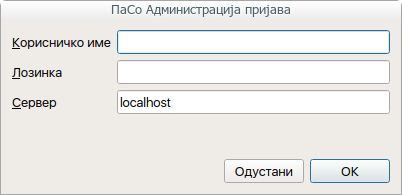
\includegraphics[scale=.5]{manual/login.png}
						\end{center}
						\caption{Пријава на систем}
						\label{figure:login_dialog}
					\end{figure}
				\end{justify}

			\newpage

			\subsection{Главни прозор}
				\begin{justify}
					По успешној пријави на систем отвориће се главни прозор у коме могу да се бирају модули које желимо да користимо. Доступност модула зависи од улоге коју корисник има, а бирају се из падајућег менија у горњем десном углу прозора.
					\begin{figure}[h]
						\begin{center}
							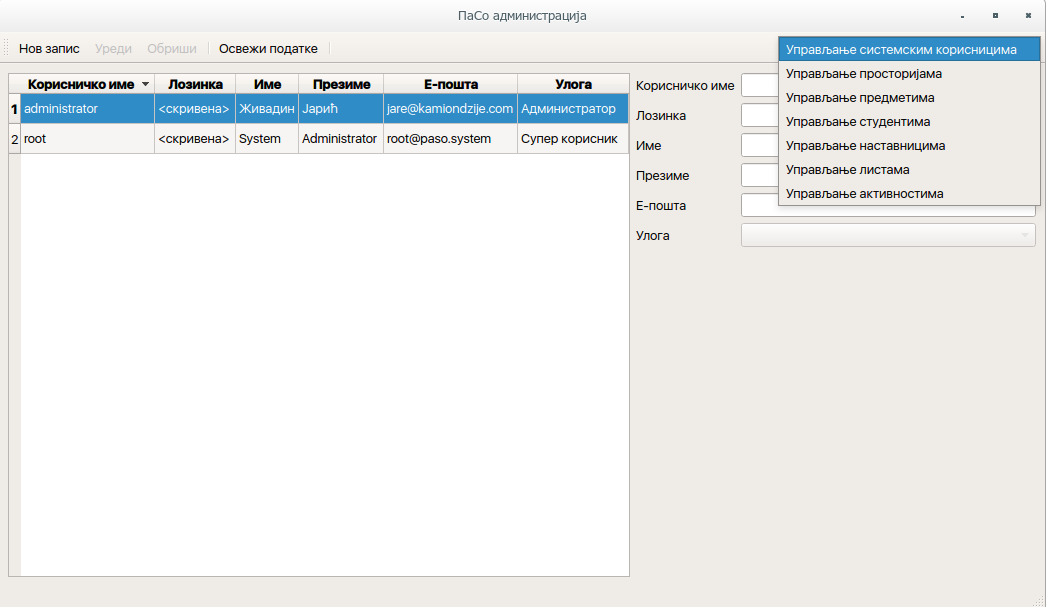
\includegraphics[width=1.0\textwidth]{manual/module_picker.png}
						\end{center}
						\caption{Одабир модула}
						\label{figure:module_picker}
					\end{figure}
				\end{justify}

			\newpage

			\subsection{Управљање системским корисницима}
				\begin{justify}
					У овом модулу вршимо комплетну администрацију системских корисника, њихов преглед, уношење, измену и брисање, а акцију коју желимо да извршимо бирамо из горње траке са алатима. Сам прозор је подељен на два дела. У левом делу стоји табеларни приказ свих системских корисника, док су у десном подаци о оном кориснику који је тренутно одабран.
					\begin{figure}[h]
						\begin{center}
							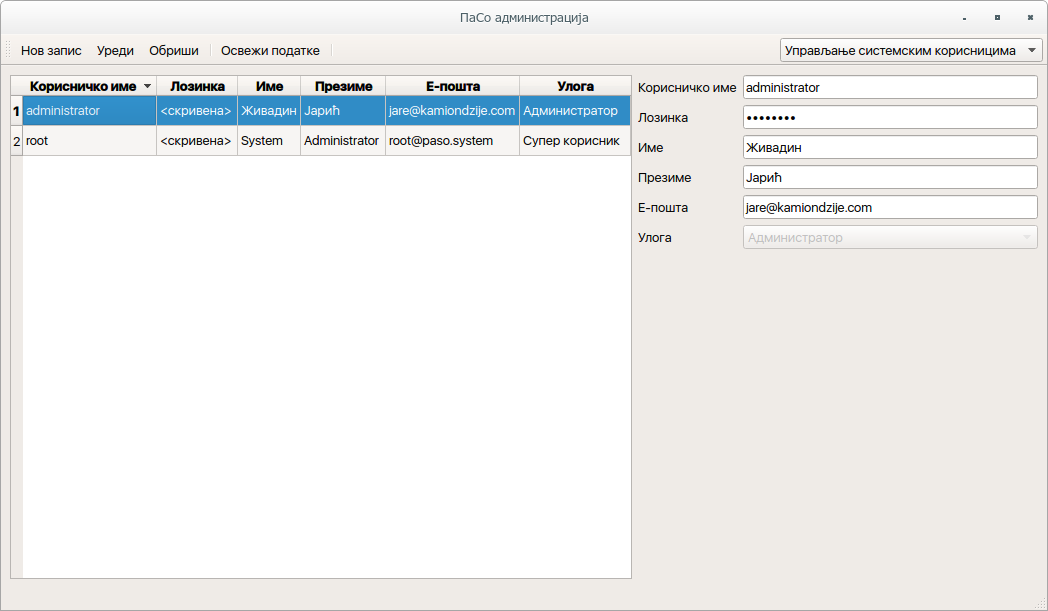
\includegraphics[width=1.0\textwidth]{manual/system_users.png}
						\end{center}
						\caption{Екран управљања системским корисницима}
						\label{figure:system_users}
					\end{figure}

					Принцип додавања, измене и брисања података, односно функционисање форме на десној страни прозора је идентично у свим модулима те ћемо га објаснити само овде, а у осталим модулима ће бити дате само специфичности везане за тај модул.

					\newpage

					По избору акције додавања новог или измене постојећег корисника, десна страна прозора ће прећи у интерактивни режим где се могу уносити подаци.
					\begin{figure}[h]
						\begin{center}
							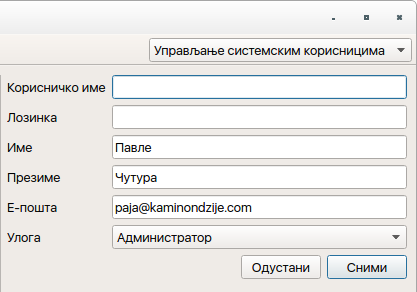
\includegraphics[width=.5\textwidth]{manual/system_user_edit.png}
						\end{center}
						\caption{Унос новог системског корисника}
						\label{figure:system_user_edit}
					\end{figure}

					Уколико неки од података нису исправни, или не задовољавају одређене критеријуме, приликом покушаја снимања систем ће вас обавестити који податак није исправан, а свако брисање захтева потврду.
					\begin{figure}[h]
						\begin{center}
							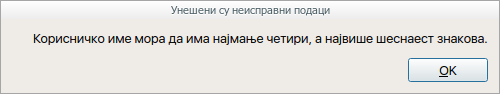
\includegraphics[width=0.75\textwidth]{manual/system_user_entry_error.png}
						\end{center}
						\caption{Обавештење о погрешном уносу података}
						\label{figure:system_user_entry_error}
					\end{figure}
					\begin{figure}[h]
						\begin{center}
							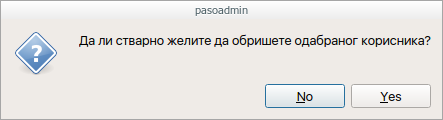
\includegraphics[width=0.75\textwidth]{manual/system_user_delete.png}
						\end{center}
						\caption{Потврда брисања корисника}
						\label{figure:system_user_delete}
					\end{figure}
				\end{justify}

			\newpage

			\subsection{Управљање просторијама}
				\begin{justify}
					Модул који обрађује просторије, је нешто компликованији пошто поред стандардне функционалности нуди преглед заузећа, могућност да се одређеним студентима експлицитно забрани улазак као и два извештаја.
					\begin{figure}[h]
						\begin{center}
							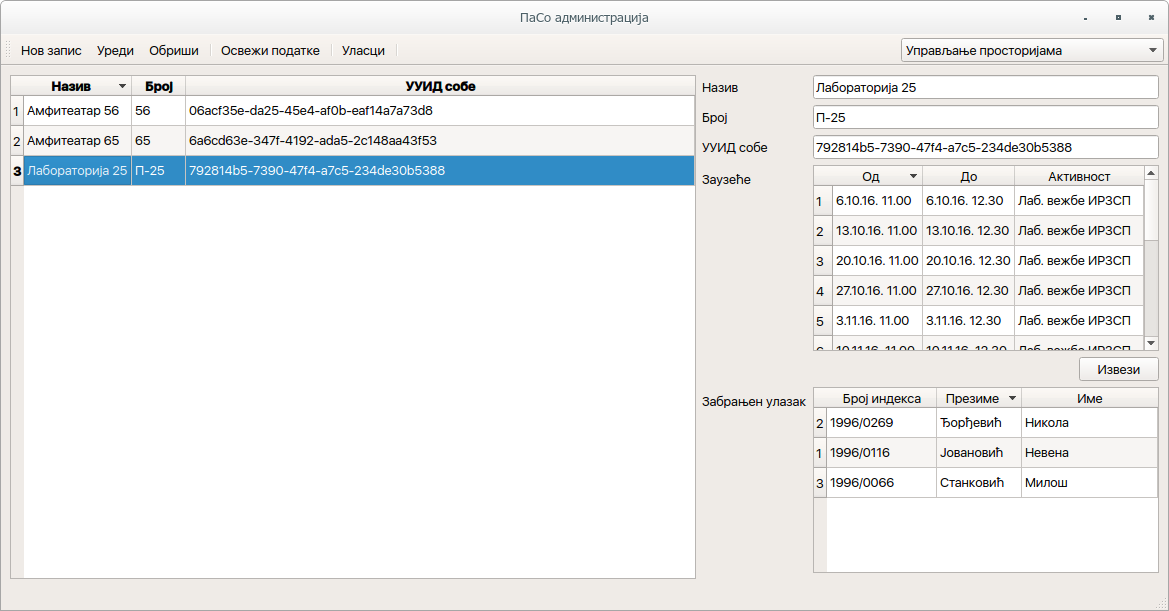
\includegraphics[width=1\textwidth]{manual/rooms_main_window.png}
						\end{center}
						\caption{Прозор управљања просторијама}
						\label{figure:rooms_main_window}
					\end{figure}\\
					Забрана уласка одређеним студентима се може мењати у режиму уређивања података о просторији кликом на дугме \quote{Измени забране}, након чега ће се отворити прозор са слике \ref{figure:room_bans} у коме се могу додавати или избацивати студенти са листе забране.
					\begin{figure}[h]
						\begin{center}
							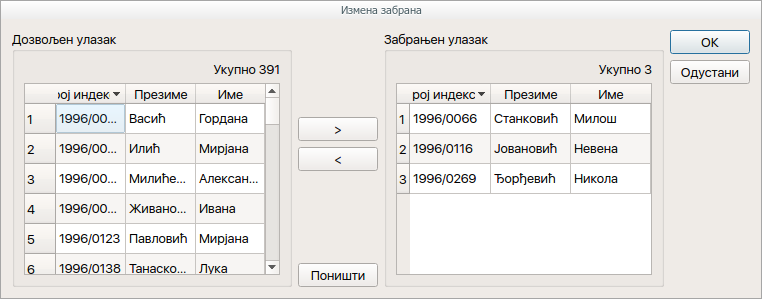
\includegraphics[width=0.9\textwidth]{manual/room_bans.png}
						\end{center}
						\caption{Прозор за уређивање забране уласка}
						\label{figure:room_bans}
					\end{figure}

					Од извештаја у овом модулу се нуди извештај заузећа просторије, који се добија кликом на дугме \quote{Извези} у десном делу где су детаљи о просторији, и извештај о уласцима у просторију за одређени временски период. Извештај о уласцима се добија одабиром акције \quote{Уласци} из главне траке са алатима која ће отворити прозор у коме се може бирати временски период који нас интересује и затражити извоз извештаја у датотеку.
					\begin{figure}[h]
						\begin{center}
							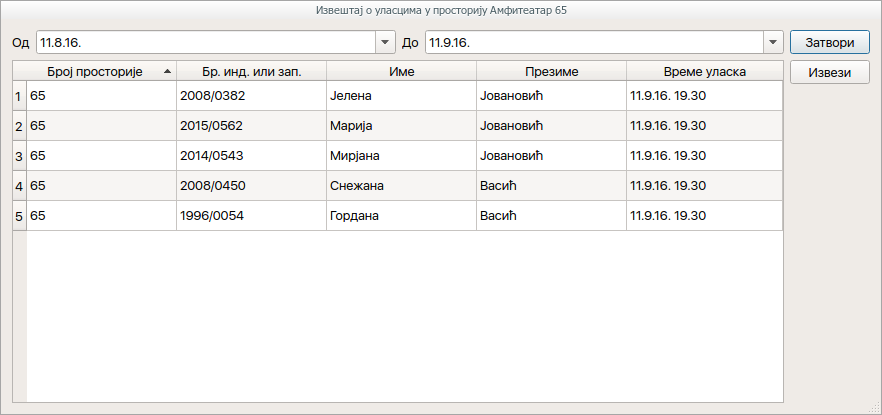
\includegraphics[width=1\textwidth]{manual/room_entries.png}
						\end{center}
						\caption{Прозор са уласцима у просторију}
						\label{figure:room_entries}
					\end{figure}

				\end{justify}
				
			\newpage

			\subsection{Управљање предметима}
				\begin{justify}
					Модул за управљање предметима, поред стандардне функционалности, додавања, измене и брисања, нуди и опције увоза списка предмета из датотека, као и могућност прегледа и измене списка студената који тај предмет слушају.
					\begin{figure}[h]
						\begin{center}
							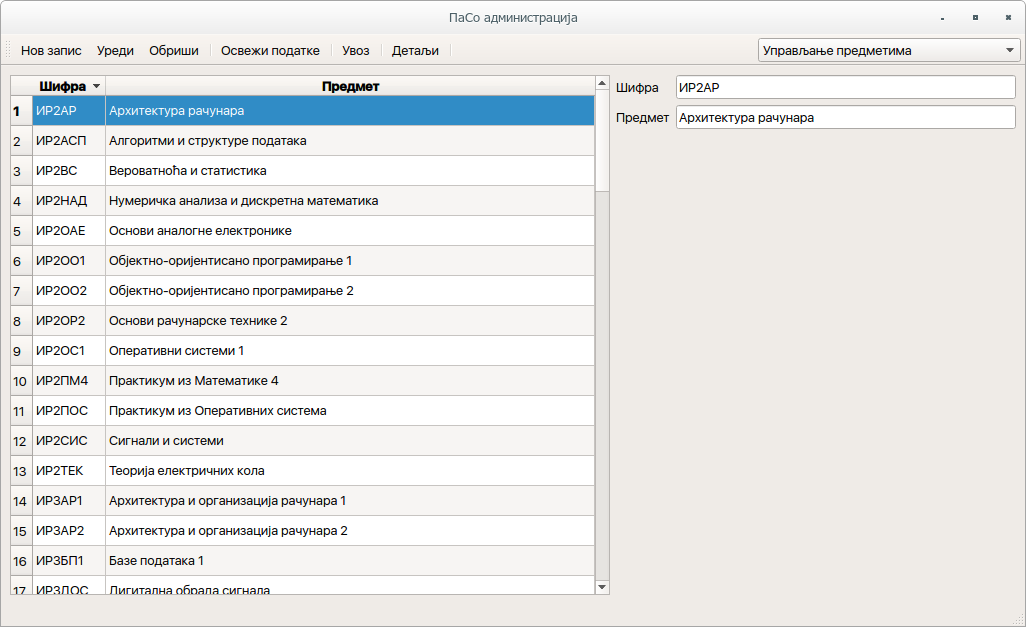
\includegraphics[width=1.0\textwidth]{manual/courses_main_window.png}
						\end{center}
						\caption{Екран управљања предметима}
						\label{figure:courses_main_window}
					\end{figure}
					Поменуте две опције се налазе у траци са алатима, као што је приказано на слици \ref{figure:courses_main_window}. Избором опције за увоз, отвориће се стандардни дијалог за одабир датотеке, а затим и прозор у коме можете видети резултате увоза података о предметима\footnote{Увоз података о предметима није деструктивна операција, већ само додаје оне предмете који нису у систему и евентуално мења назив неког од постојећих, док шифра предмета увек остаје непромењена.}.
					Одабиром опције \quote{Детаљи} отвориће се нов прозор (слика \ref{figure:courses_details_dialog}) у коме су приказани студенти који слушају и студенти који не слушају предмет. Овде се студенти могу ручно додавати и избацивати са списка, али је омогућено и да се списак студената увезе\footnote{За разлику од увоза предмета, увоз студената који слушају предмет је деструктивна операција, и стари списак ће једноставно бити замењен новим.}.

					\begin{figure}[H]
						\begin{center}
							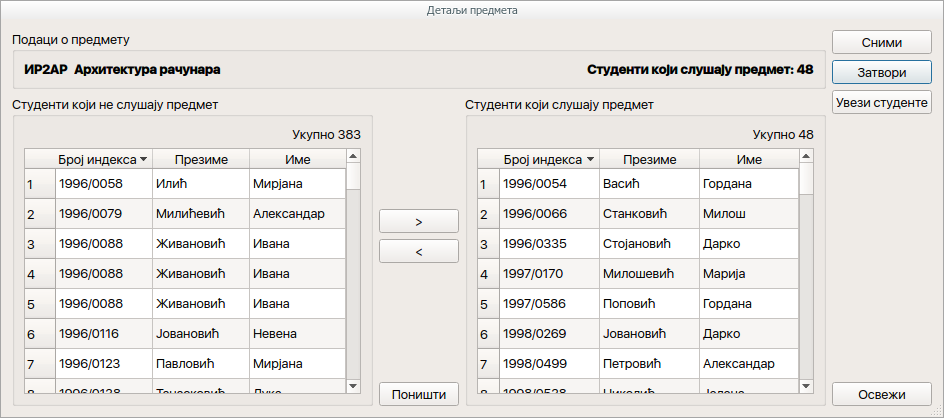
\includegraphics[width=1.0\textwidth]{manual/courses_details_dialog.png}
						\end{center}
						\caption{Детаљи предмета}
						\label{figure:courses_details_dialog}
					\end{figure}
					\begin{figure}[H]
						\begin{center}
							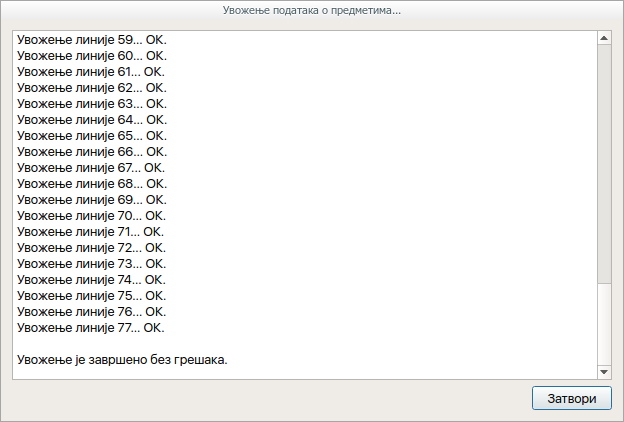
\includegraphics[width=1.0\textwidth]{manual/courses_import_dialog.png}
						\end{center}
						\caption{Извештај о увозу предмета}
						\label{figure:courses_import_dialog}
					\end{figure}
				\end{justify}

			\subsection{Управљање студентима}
				\begin{justify}
					Модул за управљање студентима омогућава администрацију података о студентима, њихов увоз путем CSV датотеке из другог система. Поред тога, могу се добити и подаци о томе које предмете студент слуша, којих је листи члан и извештај о уласцима у просторије.
					\begin{figure}[h]
						\begin{center}
							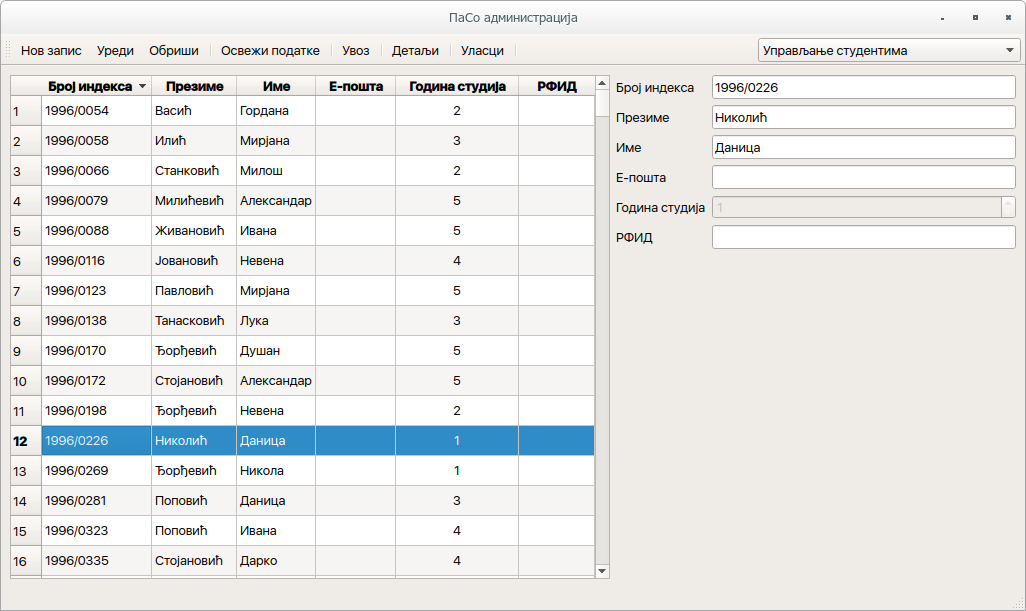
\includegraphics[width=1.0\textwidth]{manual/students_main_window.png}
						\end{center}
						\caption{Екран управљања студентима}
						\label{figure:students_main_window}
					\end{figure}
					Увоз студената је исти као увоз података о предметима, и добија се одабиром акције \quote{Увоз} из траке са алатима. По одабиру датотеке из стандардног дијалога, приказаће се прозор са резултатима увоза\footnote{Увоз студената није деструктивна операција, већ само додаје оне студенте који нису у систему и евентуално мења податке постојећих, док број индекса увек остаје непромењен.} који је исти за све операције увоза.

					Акција \quote{Детаљи} отвара нов прозор у коме се поред општих генералија студента може видети које предмете слуша и којих је листи члан, док акција \quote{Уласци} отвара нов прозор у коме се види у које је све просторије студент улазио у жељеном временском периоду. Извоз извештаја о уласцима се такође добија из овог прозора.
					\begin{figure}[H]
						\begin{center}
							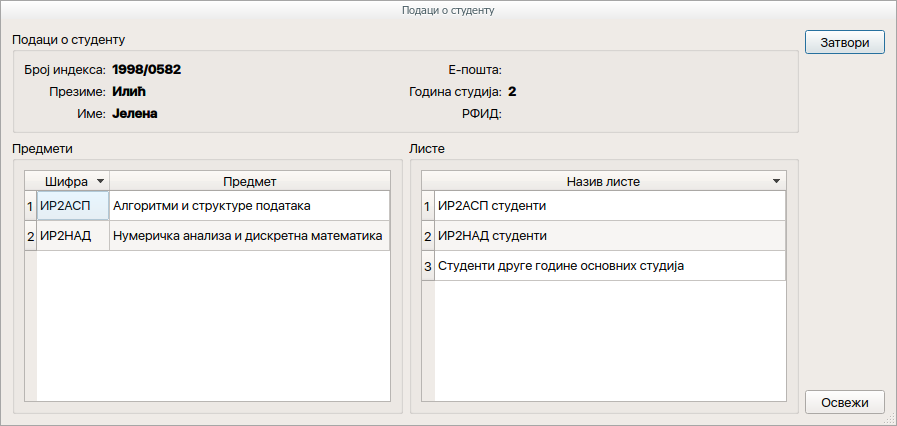
\includegraphics[width=1.0\textwidth]{manual/student_details_dialog.png}
						\end{center}
						\caption{Детаљи о студенту}
						\label{figure:student_details_dialog}
					\end{figure}
					\begin{figure}[H]
						\begin{center}
							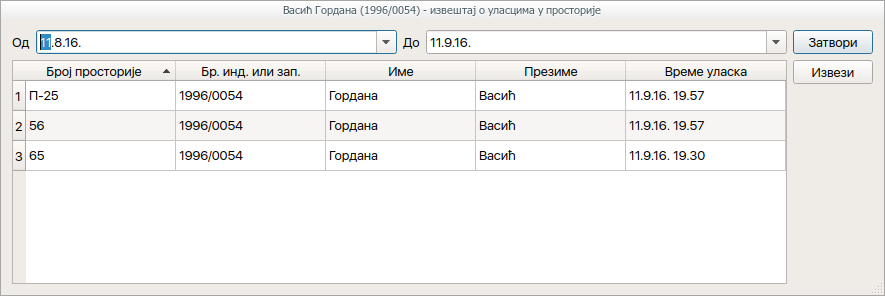
\includegraphics[width=1.0\textwidth]{manual/student_entries.png}
						\end{center}
						\caption{Извештај о уласцима студента у просторије}
						\label{figure:student_entries_dialog}
					\end{figure}
				\end{justify}

			\newpage

			\subsection{Управљање наставницима}
				\begin{justify}
					Део који се бави администрацијом наставног особља је у суштини идентичан делу који се односи на студенте, па га нећемо посебно објашњавати. Разлика је једино што код наставног особља нема детаљног прегледа, нити прегледа припадности листама јер наставници не могу да буду чланови ниједне листе.
					\begin{figure}[h]
						\begin{center}
							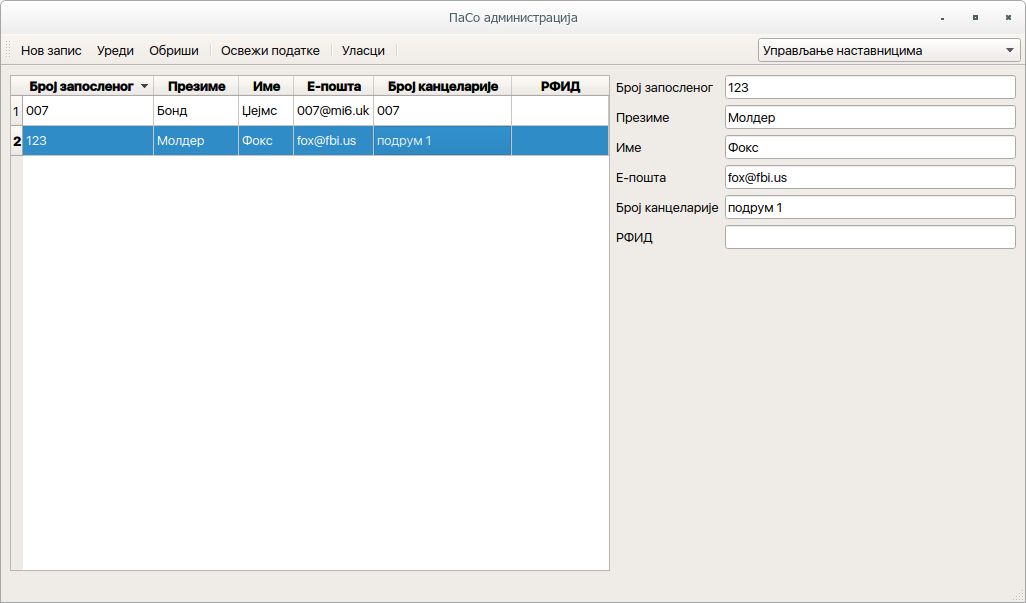
\includegraphics[width=1.0\textwidth]{manual/teachers_main_window.png}
						\end{center}
						\caption{Екран управљања наставницима}
						\label{figure:teachers_main_window}
					\end{figure}
					\begin{figure}[H]
						\begin{center}
							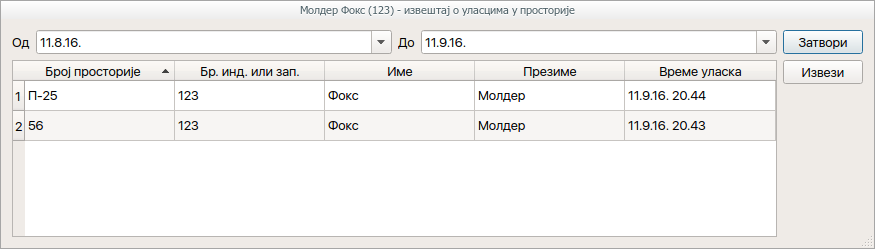
\includegraphics[width=1.0\textwidth]{manual/teacher_entries.png}
						\end{center}
						\caption{Извештај о уласцима наставника у просторије}
						\label{figure:teacher_entries}
					\end{figure}
				\end{justify}

			\newpage

			\subsection{Управљање листама}
				\begin{justify}
					Екран на коме се ради администрација листи је приказан на слици \ref{figure:lists_main_window}. Овај екран поред стандардне функционалности нуди и акцију \quote{Детаљи} која отвара нови прозор у коме можемо да манипулишемо члановима листи. Поред ручног додавања и избацивања студената из листе, могућ је и увоз који функционише на идентичан начин као код увоза студената који слушају неки предмет\footnote{Ова операција је, као и што је и операција увоза студената који слушају неки предмет, деструктивна и једноставно ће заменити текући списак студената новим.}.
					\begin{figure}[h]
						\begin{center}
							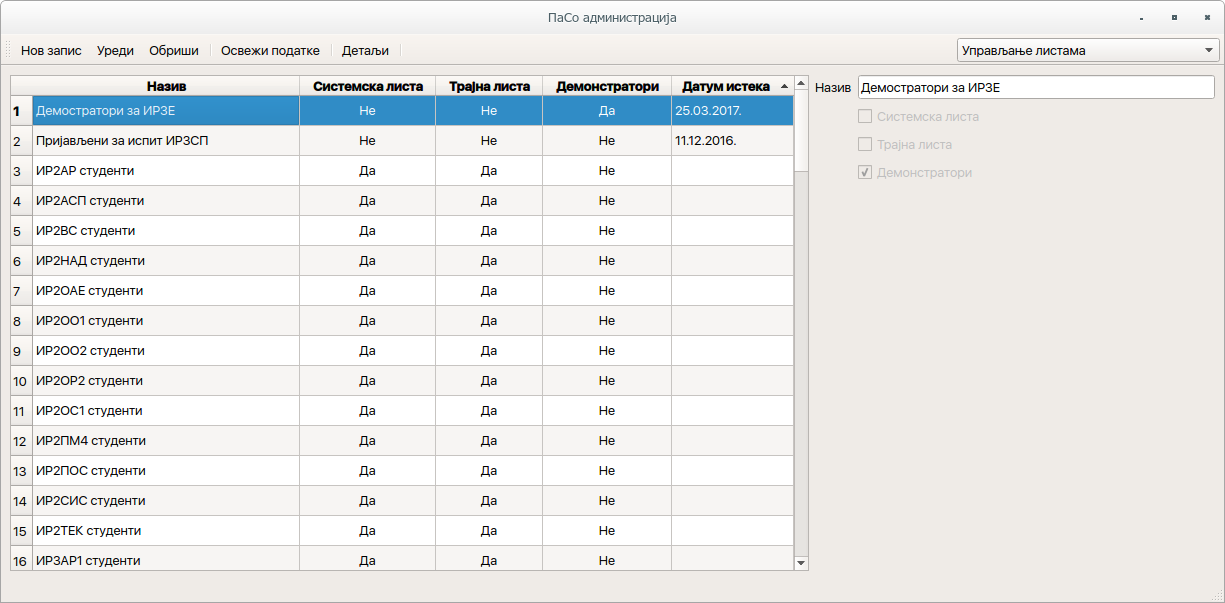
\includegraphics[width=1.0\textwidth]{manual/lists_main_window.png}
						\end{center}
						\caption{Екран управљања листама}
						\label{figure:lists_main_window}
					\end{figure}
					Уколико је листа системска онда измена података није могућа.
					\begin{figure}[h]
						\begin{center}
							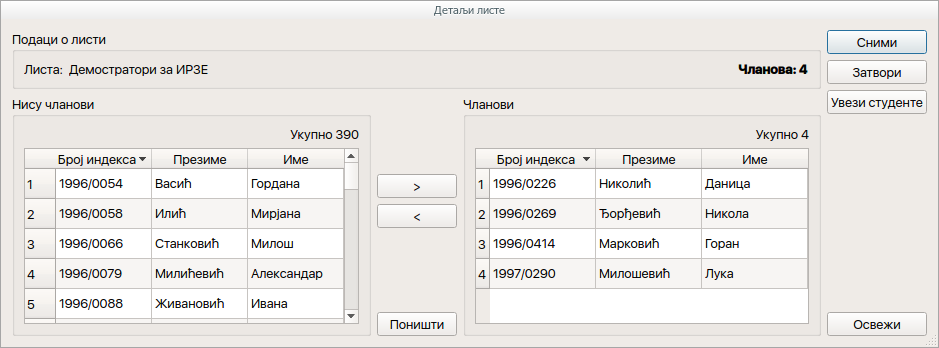
\includegraphics[width=.95\textwidth]{manual/list_details_dialog.png}
						\end{center}
						\caption{Детаљи листе}
						\label{figure:list_details_dialog}
					\end{figure}
				\end{justify}

			\newpage

			\subsection{Управљање активностима}
				\begin{justify}
					Активности су вероватно најважнији део целог система па због своје сложености и количине података коју носе, екран за управљање њима нема могућност директног уређивања, већ се оно врши низом корака уз помоћ чаробњака.
					\begin{figure}[h]
						\begin{center}
							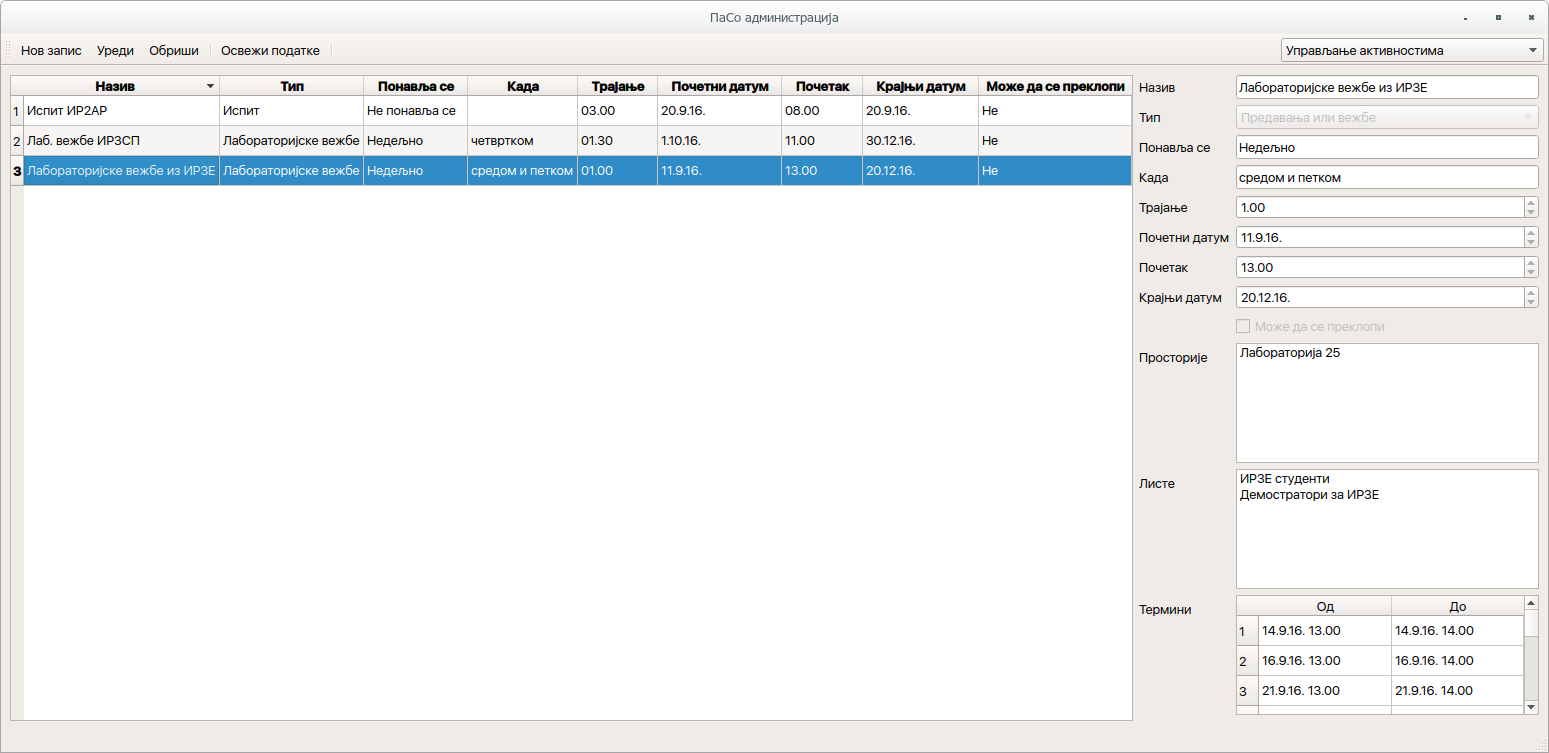
\includegraphics[width=1.0\textwidth]{manual/activities_main_window.png}
						\end{center}
						\caption{Екран управљања листама}
						\label{figure:activities_main_window}
					\end{figure}\\
					\noindent
					Кораци односно странице којима се иде кроз чаробњак су следећи:
					\begin{enumerate}[noitemsep]
						\item Унос имена, одабир врсте, као и периодичности.
						\item Унос времена и трајања, или одабир када се активност понавља.
						\item Везивање листи студената за активност.
						\item Избор просторија у којима ће се активност обављати.
					\end{enumerate}
					Други корак се разликује у зависности од избора које корисник направи на првој страници чаробњака. Уколико је одабрано да се активност не понавља, други корак се своди на одабир датума и времена почетка активности као и њеног трајања. Ако се активност понавља, на недељном или месечном нивоу, онда се ради одабир почетка и краја периода, време трајања појединачне активности, време њеног почетка, као и дани у недељи односно датуми у месецу када се понавља. Ово је илустровано на сликама \ref{figure:single_time} и \ref{figure:multiple_time}.
					Уколико је активност посебног типа, као што су рецимо конференције или јавна предавања и трибине, корак одабира листи се прескаче.

					Када је корисник завршио све кораке, приликом покушаја снимања активности, ако има преклапања термина за било коју просторију са било којом активношћу изузев активности типа \quote{Индивидуални рад} корисник ће бити обавештен, моћи ће да прегледа која су преклапања и да одлучи хоће ли да сними активност или да се врати на чаробњака (слике \ref{figure:overlap_warning} и \ref{figure:overlaps}).

					\begin{figure}[H]
						\begin{center}
							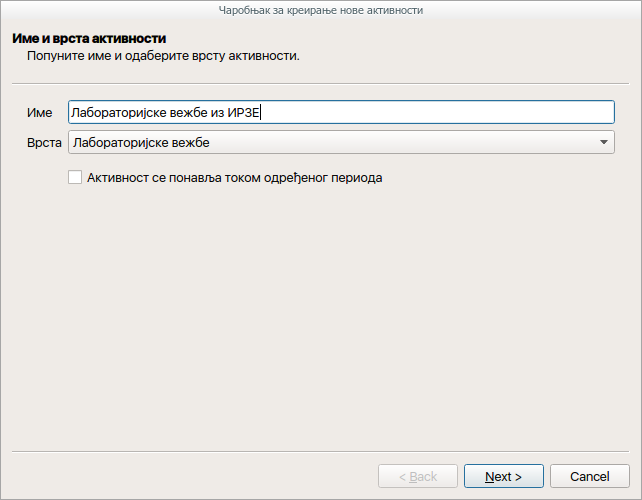
\includegraphics[width=0.70\textwidth]{manual/activity_wizard_name_and_type.png}
						\end{center}
						\caption{Унос имена и врсте активности која се не понавља}
						\label{figure:single_name_and_type}
					\end{figure}
					\begin{figure}[H]
						\begin{center}
							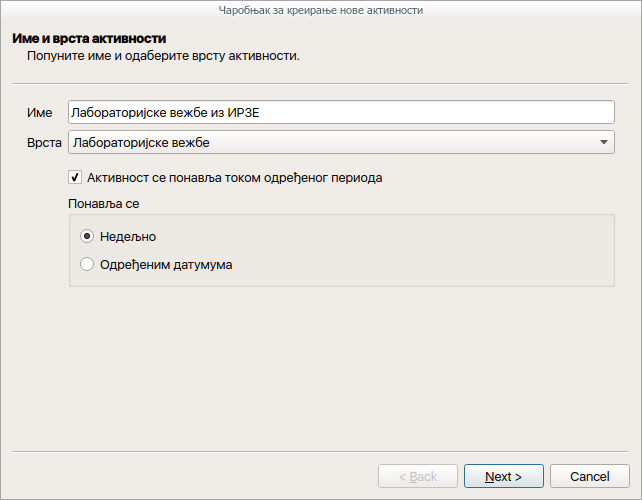
\includegraphics[width=0.70\textwidth]{manual/activity_wizard_name_and_type_repetitive.png}
						\end{center}
						\caption{Унос имена и врсте активности која се понавља}
						\label{figure:repetitive_name_and_type}
					\end{figure}
					\begin{figure}[H]
						\begin{center}
							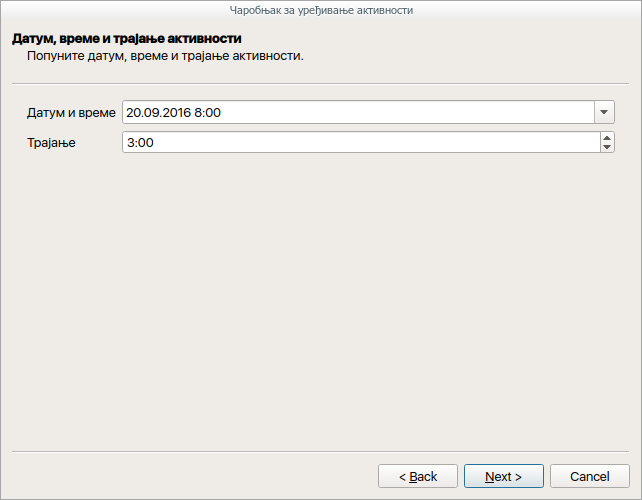
\includegraphics[width=0.70\textwidth]{manual/activity_wizard_time.png}
						\end{center}
						\caption{Време и трајање активности која се не понавља}
						\label{figure:single_time}
					\end{figure}
					\begin{figure}[H]
						\begin{center}
							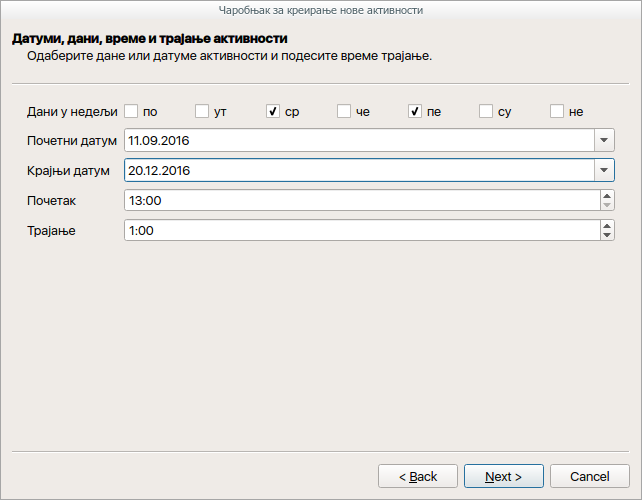
\includegraphics[width=0.70\textwidth]{manual/activity_wizard_time_slots.png}
						\end{center}
						\caption{Време и трајање активност која се понавља}
						\label{figure:multiple_time}
					\end{figure}
					\begin{figure}[H]
						\begin{center}
							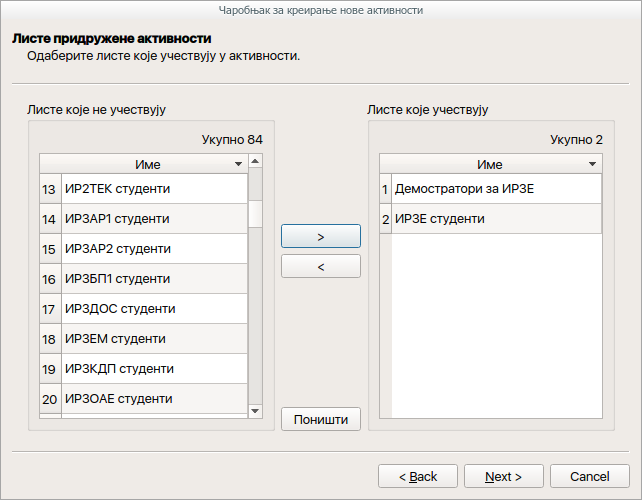
\includegraphics[width=0.70\textwidth]{manual/activity_wizard_lists.png}
						\end{center}
						\caption{Одабир листи које су везане за активност}
						\label{figure:activity_lists}
					\end{figure}
					\begin{figure}[H]
						\begin{center}
							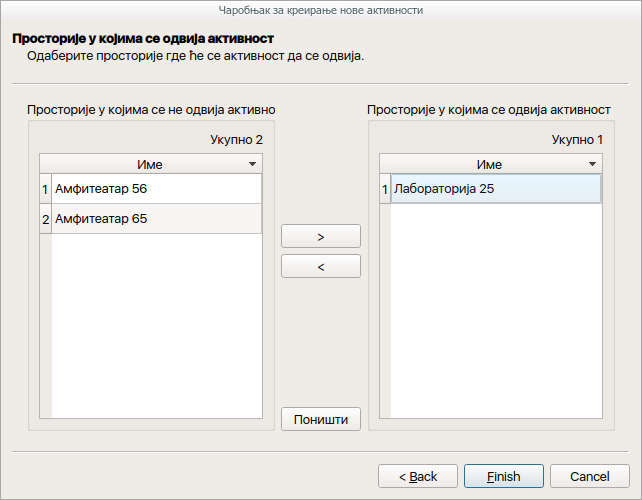
\includegraphics[width=0.70\textwidth]{manual/activity_wizard_rooms.png}
						\end{center}
						\caption{Одабир просторија у којима ће се одвијати активност}
						\label{figure:activity_rooms}
					\end{figure}
					\begin{figure}[H]
						\begin{center}
							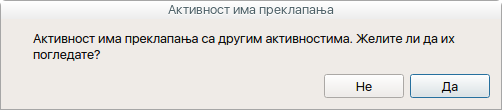
\includegraphics[width=0.70\textwidth]{manual/overlap_warning.png}
						\end{center}
						\caption{Обавештење да активност има преклапања}
						\label{figure:overlap_warning}
					\end{figure}
					\begin{figure}[H]
						\begin{center}
							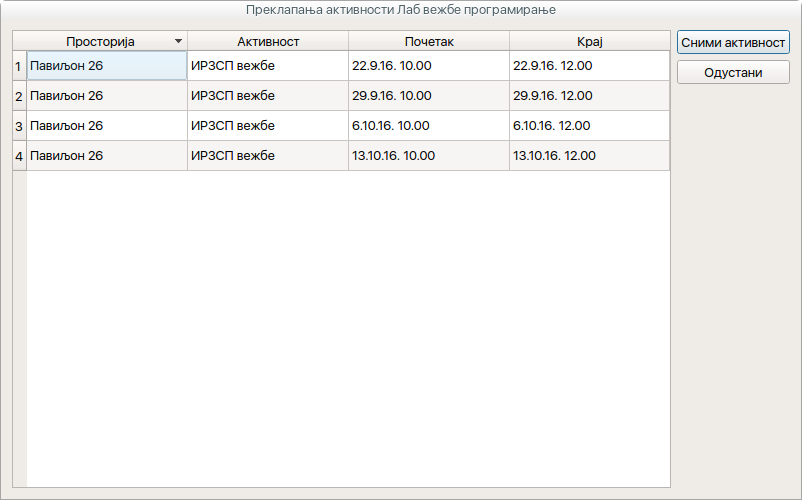
\includegraphics[width=0.70\textwidth]{manual/overlaps.png}
						\end{center}
						\caption{Преглед преклапања активности}
						\label{figure:overlaps}
					\end{figure}
				\end{justify}

		\newpage

		\section{Симулатор}
			\begin{justify}
				Симулатор контролера просторије је графичка апликација и представља добру алатку за илустровање рада система, и још важније може врло ефикасно да служи као испомоћ за отклањање грешака у комуникацији између сервера и контролера просторија.

				Симулатор се покреће извршавањем команде \textbf{pasosimulator} и након тога ће се отворити прозор који изгледа као на слици \ref{figure:simulator_main_window}.
				\begin{figure}[h]
					\begin{center}
						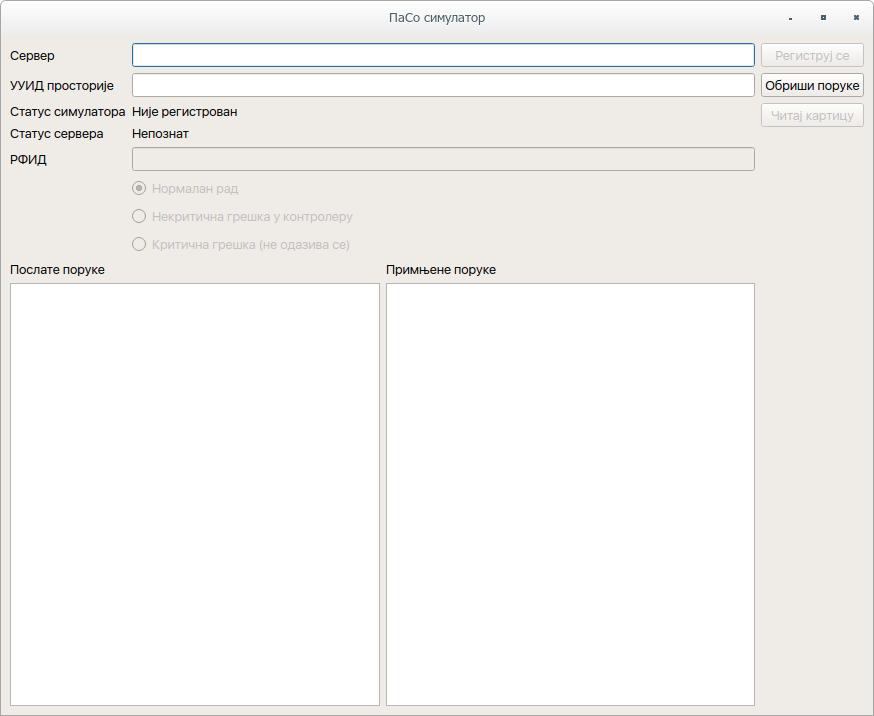
\includegraphics[width=1.0\textwidth]{manual/simulator_main_window.png}
					\end{center}
					\caption{Прозор симулатора}
					\label{figure:simulator_main_window}
				\end{figure}
				У доњем делу прозора постоје два поља у којима се могу пратити поруке које симулатор шаље серверу и поруке које прима од сервера. Функције и значење осталих контрола биће објашњене даље у тексту.

				Да би се почело коришћење симулатора потребно је попунити поља \quote{Сервер} и \quote{УУИД просторије} и притиснути дугме \quote{Региструј се}. Након тога ће симулатор контактирати сервер и захтевати регистрацију. По успешној регистрацији, остале контроле ће бити укључене, а у доњем делу ћемо видети поруке које су разменили симулатор и сервер, што се види на слици \ref{figure:simulator_registered}.
				\begin{figure}[H]
					\begin{center}
						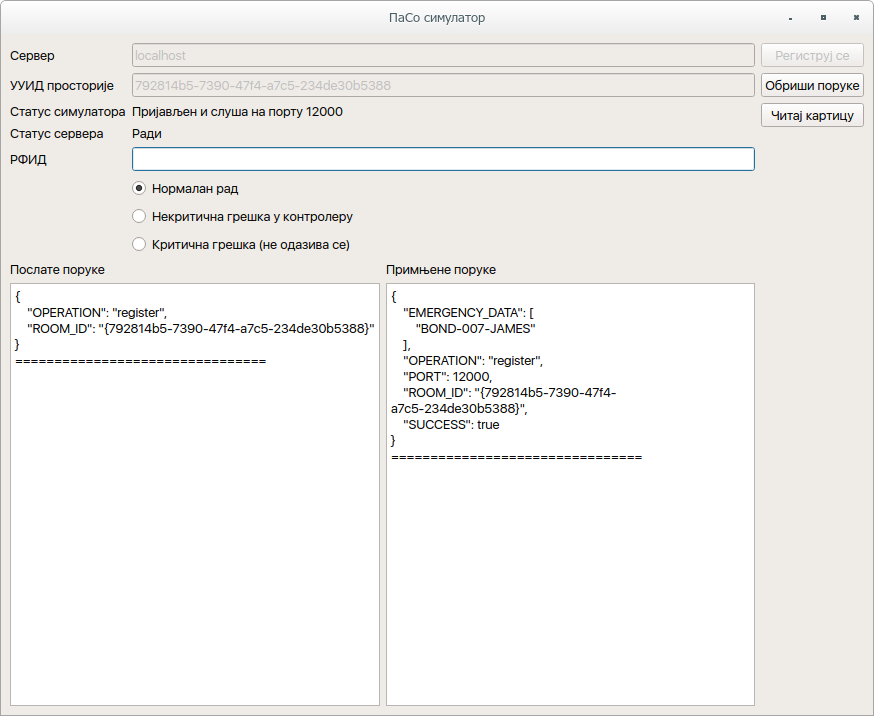
\includegraphics[width=1.0\textwidth]{manual/simulator_registered.png}
					\end{center}
					\caption{Изглед симулатора по регистрацији на сервер}
					\label{figure:simulator_registered}
				\end{figure}
				У поље \quote{РФИД} се уноси РФ идентификатор студентске или професорске картице који смо задали у административној конзоли, док дугмад испод служе за симулирање отказа контролера.
				Изнад \quote{РФИД} поља се налазе статуси сервера и контролера где можемо да видимо и на ком порту је сервер захтевао да контролер слуша. Комуникацију са симулираним отказом можемо видети на слици \ref{figure:simulator_failure}. Ако је укључено дугме \quote{Критична грешка} симулатор се уопште неће одазивати, и то би требало да резултује записима у серверски дневник.
				\begin{figure}[H]
					\begin{center}
						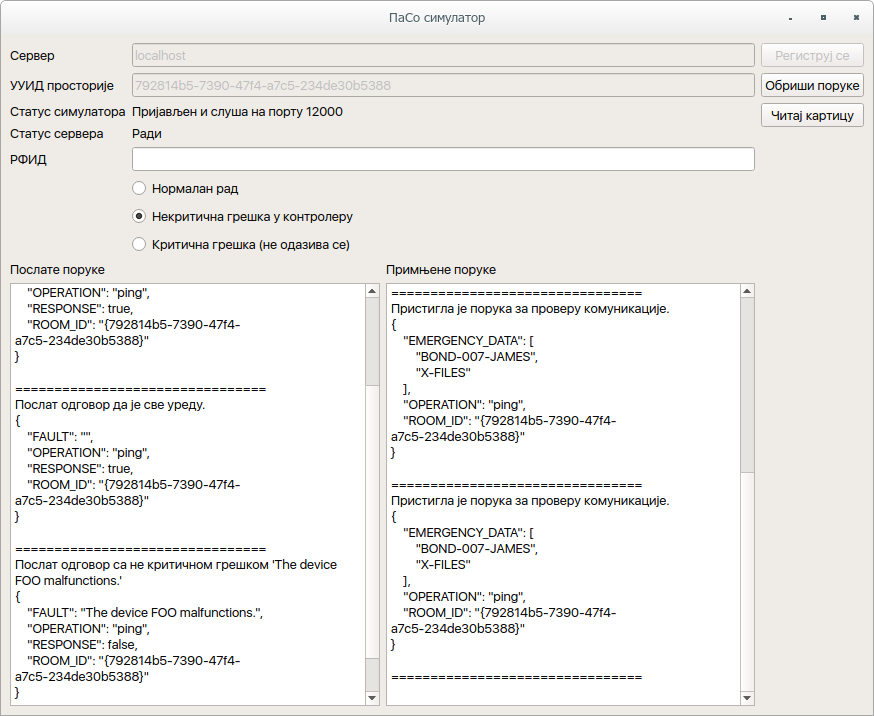
\includegraphics[width=1.0\textwidth]{manual/simulator_failure.png}
					\end{center}
					\caption{Изглед комуникације са симулираним не критичним отказом}
					\label{figure:simulator_failure}
				\end{figure}

				Након успешне регистрације у поље \quote{РФИД} је потребно унети вредност која је придружена неком од студената или професора и притиснути дугме \quote{Читај картицу} како би симулирали улазак у просторију. Уколико је у питању студент, и у току је нека активност којој би он требало да присуствује, сервер ће одговорити потврдно. На слици \ref{figure:simulator_read} се види одбијен приступ студенту и дат приступ професору.
				\begin{figure}[H]
					\begin{center}
						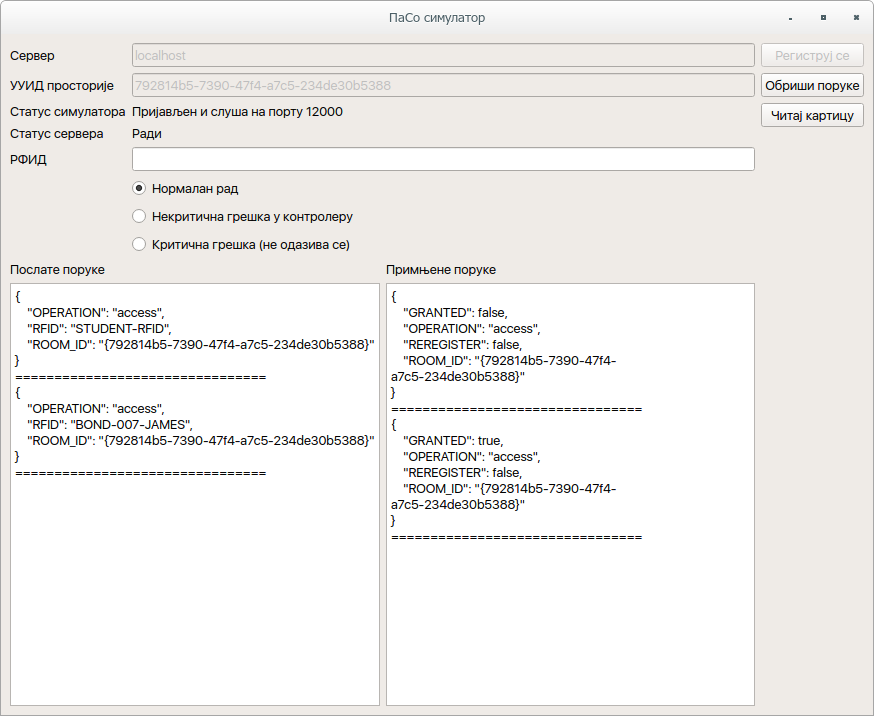
\includegraphics[width=1.0\textwidth]{manual/simulator_card_read.png}
					\end{center}
					\caption{Изглед комуникације при датом и одбијеном приступу}
					\label{figure:simulator_read}
				\end{figure}

				Да би се омогућило симулирање система са више просторија, може се покренути произвољан број симулатора, а сервер ће сваком од њих доделити други порт. За што бољи увид и то шта се дешава у систему, симулатор је најбоље користити уз истовремено праћење серверског дневника.

			\end{justify}

	\begin{thebibliography}{9}
		\bibitem{qt_website}
		The Qt Company, \quote{Qt Documentation},
		http://doc.qt.io

		\bibitem{cplusplus}
		cplusplus.com, \quote{C++ Reference},
		http://www.cplusplus.com/reference

		\bibitem{postgresql}
		PostgreSQL, \quote{Documentation},
		https://www.postgresql.org/docs

		\bibitem{jsonschema}
		JSON Schema and Hyper-Schema, \quote{Documentation},\\
		http://json-schema.org/documentation.html

		\bibitem{pragprog}
		Andrew Hunt, David Thomas, \quote{The Pragmatic Programmer: From Journeyman to Master},
		прво издање, The Pragmatic Bookshelf, 1999, ИСБН 978-0-2016-1622-4

		\bibitem{tddcpp}
		Jeff Langr, \quote{Modern C++ Programming with Test-Driven Development: Code Better, Sleep Better},
		прво издање, The Pragmatic Bookshelf, 2013, ИСБН 978-1-937785-48-2

		\bibitem{cmake}
		CMake.org, \quote{Documentation},
		https://cmake.org/documentation/

		\bibitem{thelatex}
		The \LaTeX Project, \quote{LaTeX Documentation},\\
		https://www.latex-project.org/help/documentation/

		\bibitem{doxygen}
		Doxygen, \quote{Doxygen Manual},
		http://www.stack.nl/~dimitri/doxygen/manual/index.html

		\bibitem{openssl}
		OpenSSL, \quote{OpenSSL Docs},
		https://www.openssl.org/docs/
	\end{thebibliography}
\end{document}